%% We use the memoir class because it offers a many easy to use features.
\documentclass[10pt,a4paper,titlepage,openany,oneside]{memoir}

%% `usepackage` commands.
%% Packages
%% ========

%% LaTeX Font encoding -- DO NOT CHANGE
\usepackage[OT1]{fontenc}

%% Babel provides support for languages.  'english' uses British
%% English hyphenation and text snippets like "Figure" and
%% "Theorem". Use the option 'ngerman' if your document is in German.
%% Use 'american' for American English.  Note that if you change this,
%% the next LaTeX run may show spurious errors.  Simply run it again.
%% If they persist, remove the .aux file and try again.
\usepackage[english]{babel}

%% Input encoding 'utf8'. In some cases you might need 'utf8x' for
%% extra symbols. Not all editors, especially on Windows, are UTF-8
%% capable, so you may want to use 'latin1' instead.
\usepackage[utf8]{inputenc}

%% This changes default fonts for both text and math mode to use Herman Zapfs
%% excellent Palatino font. Do not change this.
\usepackage[sc]{mathpazo}

%% The AMS-LaTeX extensions for mathematical typesetting.  Do not
%% remove.
\usepackage{amsmath,amssymb,amsfonts,mathrsfs}
\allowdisplaybreaks

%% NTheorem is a reimplementation of the AMS Theorem package. This
%% will allow us to typeset theorems like examples, proofs and
%% similar.  Do not remove.
%% NOTE: Must be loaded AFTER amsmath, or the \qed placement will
%% break
\usepackage[amsmath,thmmarks]{ntheorem}

%% LaTeX' own graphics handling
\usepackage{graphicx}

%% We unfortunately need this for the Rules chapter.  Remove it
%% afterwards; or at least NEVER use its underlining features.
\usepackage{soul}

%% This allows you to add .pdf files. It is used to add the
%% declaration of originality.
\usepackage{pdfpages}

%% Extra Packages
%% ==============

%% [OPT] Multi-rowed cells in tabulars
%\usepackage{multirow}

%% [REC] Intelligent cross reference package. This allows for nice
%% combined references that include the reference and a hint to where
%% to look for it.
\usepackage{varioref}

%% [OPT] Easily changeable quotes with \enquote{Text}
%\usepackage[german=swiss]{csquotes}

%% [REC] Format dates and time depending on locale
\usepackage{datetime}

%% [OPT] Provides a \cancel{} command to stroke through mathematics.
%\usepackage{cancel}

%% [NEED] This allows for additional typesetting tools in mathmode.
%% See its excellent documentation.
\usepackage{mathtools}

%% [ADV] Conditional commands
%\usepackage{ifthen}

%% [OPT] Manual large braces or other delimiters.
%\usepackage{bigdelim, bigstrut}

%% [REC] Alternate vector arrows. Use the command \vv{} to get scaled
%% vector arrows.
\usepackage[h]{esvect}

%% [NEED] Some extensions to tabulars and array environments.
\usepackage{array}

%% [OPT] Postscript support via pstricks graphics package. Very
%% diverse applications.
%\usepackage{pstricks,pst-all}

%% [?] This seems to allow us to define some additional counters.
%\usepackage{etex}

%% [ADV] XY-Pic to typeset some matrix-style graphics
%\usepackage[all]{xy}

%% [OPT] This is needed to generate an index at the end of the
%% document.
%\usepackage{makeidx}

%% [OPT] Fancy package for source code listings.  The template text
%% needs it for some LaTeX snippets; remove/adapt the \lstset when you
%% remove the template content.
\usepackage{listings}
\lstset{language=TeX,basicstyle={\normalfont\ttfamily}}

%% [REC] Fancy character protrusion.  Must be loaded after all fonts.
\usepackage[activate]{pdfcprot}

%% [REC] Nicer tables.  Read the excellent documentation.
\usepackage{booktabs}

%% Fancy Enumeration environment
\usepackage{enumitem}

%% Bibliography package.
\usepackage[
style=authoryear,
sorting=ynt,
natbib=true,
mincitenames=1,
maxcitenames=2,
backend=biber]{biblatex}
\addbibresource{reference.bib}

%% Side-by-Side Figures
\usepackage{caption}
\usepackage{subcaption}

%% Bold math symbols.
\usepackage{bm}
\usepackage{bbm}

%% Color for table cells.
\usepackage{xcolor,colortbl}

%% Table multiple rows.
\usepackage{multirow}

%% Algorithms environment
\usepackage[ruled,vlined,linesnumbered,noresetcount]{algorithm2e}

%% Force Figures to not float out of Section
\usepackage{float}

%% API
%% ===

%% Make document internal hyperlinks wherever possible. (TOC, references)
%% This MUST be loaded after varioref. We just load it last to be safe.
\usepackage[
linkcolor=black,
colorlinks=true,
citecolor=black,
filecolor=black]{hyperref}

% \let\oldcitet=\citet
% \let\oldcitep=\citep 
% \renewcommand{\citet}[1]{\textcolor[rgb]{0,0,1}{\oldcitet{#1}}}
% \renewcommand{\citep}[1]{\textcolor[rgb]{0,0,1}{\oldcitep{#1}}}

%% Our layout configuration.
%% Memoir layout setup

%% NOTE: You are strongly advised not to change any of them unless you
%% know what you are doing.  These settings strongly interact in the
%% final look of the document.

% Turn extra space before chapter headings off.
\setlength{\beforechapskip}{0pt}

\nonzeroparskip
\parindent=0pt
\defaultlists

% Chapter style redefinition
\makeatletter

\if@twoside
  \pagestyle{Ruled}
  \copypagestyle{chapter}{Ruled}
\else
  \pagestyle{ruled}
  \copypagestyle{chapter}{ruled}
\fi
\makeoddhead{chapter}{}{}{}
\makeevenhead{chapter}{}{}{}
\makeheadrule{chapter}{\textwidth}{0pt}
\copypagestyle{abstract}{empty}

\makechapterstyle{bianchimod}{%
  \chapterstyle{default}
  \renewcommand*{\chapnamefont}{\normalfont\Large\sffamily}
  \renewcommand*{\chapnumfont}{\normalfont\Large\sffamily}
  \renewcommand*{\printchaptername}{%
    \chapnamefont\centering\@chapapp}
  \renewcommand*{\printchapternum}{\chapnumfont {\thechapter}}
  \renewcommand*{\chaptitlefont}{\normalfont\huge\sffamily}
  \renewcommand*{\printchaptertitle}[1]{%
    \hrule\vskip\onelineskip \centering \chaptitlefont\textbf{\vphantom{gyM}##1}\par}
  \renewcommand*{\afterchaptertitle}{\vskip\onelineskip \hrule\vskip
    \afterchapskip}
  \renewcommand*{\printchapternonum}{%
    \vphantom{\chapnumfont {9}}\afterchapternum}}

% Use the newly defined style
\chapterstyle{bianchimod}

\setsecheadstyle{\Large\bfseries\sffamily}
\setsubsecheadstyle{\large\bfseries\sffamily}
\setsubsubsecheadstyle{\bfseries\sffamily}
\setparaheadstyle{\normalsize\bfseries\sffamily}
\setsubparaheadstyle{\normalsize\itshape\sffamily}
\setsubparaindent{0pt}

% Set captions to a more separated style for clearness
\captionnamefont{\sffamily\bfseries\footnotesize}
\captiontitlefont{\sffamily\footnotesize}
\setlength{\intextsep}{12pt}
\setlength{\belowcaptionskip}{1pt}

% Set section and TOC numbering depth to subsection
\setsecnumdepth{subsection}
\settocdepth{subsection}

%% Titlepage adjustments
\pretitle{\vspace{0pt plus 0.7fill}\begin{center}\HUGE\sffamily\bfseries}
\posttitle{\end{center}\par}
\preauthor{\par\begin{center}\let\and\\\Large\sffamily}
\postauthor{\end{center}}
\predate{\par\begin{center}\Large\sffamily}
\postdate{\end{center}}

\def\@advisors{}
\newcommand{\advisors}[1]{\def\@advisors{#1}}
\def\@department{}
\newcommand{\department}[1]{\def\@department{#1}}
\def\@thesistype{}
\newcommand{\thesistype}[1]{\def\@thesistype{#1}}

\renewcommand{\maketitlehooka}{\noindent\logo[2.5in]}

\renewcommand{\maketitlehookb}{\vspace{1in}%
  \par\begin{center}\Large\sffamily\@thesistype\end{center}}

\renewcommand{\maketitlehookd}{%
  \vfill\par
  \begin{flushright}
    \sffamily
    \@advisors\par
    \@department, Imperial College London
  \end{flushright}
}

\checkandfixthelayout

\setlength{\droptitle}{-35pt} %-48

\makeatother

% This defines how theorems should look. Best leave as is.
\theoremstyle{plain}
\setlength\theorempostskipamount{0pt}

%%% Local Variables:
%%% mode: latex
%%% TeX-master: "thesis"
%%% End:


%% Theorem environments.
%% Theorem-like environments

\numberwithin{equation}{chapter}

%% English variants
\newtheorem{theorem}{Theorem}[chapter]
\newtheorem{example}[theorem]{Example}
\newtheorem{remark}[theorem]{Remark}
\newtheorem{corollary}[theorem]{Corollary}
\newtheorem{definition}[theorem]{Definition}
\newtheorem{lemma}[theorem]{Lemma}
\newtheorem{proposition}[theorem]{Proposition}
\newtheorem{hypothesis}[theorem]{Hypothesis}
\newtheorem{assumption}[theorem]{Assumption}

%% Proof environment with a small square as a "qed" symbol
\theoremstyle{nonumberplain}
\theorembodyfont{\normalfont}
\theoremsymbol{\ensuremath{\square}}
\newtheorem{proof}{Proof}
%\newtheorem{beweis}{Beweis}


%% Helpful macros.
%% Custom commands
%% ===============

%% logo command
\newcommand{\logo}[1][\textwidth]{\resizebox{#1}{!}{
\includegraphics{setup/logo}}}

%% Ian Goodfellow LaTeX commands for math.
%%%%% NEW MATH DEFINITIONS %%%%%



\def\ceil#1{\lceil #1 \rceil}
\def\floor#1{\lfloor #1 \rfloor}
\def\1{\bm{1}}
\newcommand{\train}{\mathcal{D}}
\newcommand{\valid}{\mathcal{D_{\mathrm{valid}}}}
\newcommand{\test}{\mathcal{D_{\mathrm{test}}}}

\def\eps{{\epsilon}}


% Random variables
\def\reta{{\textnormal{$\eta$}}}
\def\ra{{\textnormal{a}}}
\def\rb{{\textnormal{b}}}
\def\rc{{\textnormal{c}}}
\def\rd{{\textnormal{d}}}
\def\re{{\textnormal{e}}}
\def\rf{{\textnormal{f}}}
\def\rg{{\textnormal{g}}}
\def\rh{{\textnormal{h}}}
\def\ri{{\textnormal{i}}}
\def\rj{{\textnormal{j}}}
\def\rk{{\textnormal{k}}}
\def\rl{{\textnormal{l}}}
%\def\rm{{\textnormal{m}}}
\def\rn{{\textnormal{n}}}
\def\ro{{\textnormal{o}}}
\def\rp{{\textnormal{p}}}
\def\rq{{\textnormal{q}}}
\def\rr{{\textnormal{r}}}
\def\rs{{\textnormal{s}}}
\def\rt{{\textnormal{t}}}
\def\ru{{\textnormal{u}}}
\def\rv{{\textnormal{v}}}
\def\rw{{\textnormal{w}}}
\def\rx{{\textnormal{x}}}
\def\ry{{\textnormal{y}}}
\def\rz{{\textnormal{z}}}

% Random vectors
\def\rvepsilon{{\mathbf{\epsilon}}}
\def\rvtheta{{\mathbf{\theta}}}
\def\rva{{\mathbf{a}}}
\def\rvb{{\mathbf{b}}}
\def\rvc{{\mathbf{c}}}
\def\rvd{{\mathbf{d}}}
\def\rve{{\mathbf{e}}}
\def\rvf{{\mathbf{f}}}
\def\rvg{{\mathbf{g}}}
\def\rvh{{\mathbf{h}}}
\def\rvu{{\mathbf{i}}}
\def\rvj{{\mathbf{j}}}
\def\rvk{{\mathbf{k}}}
\def\rvl{{\mathbf{l}}}
\def\rvm{{\mathbf{m}}}
\def\rvn{{\mathbf{n}}}
\def\rvo{{\mathbf{o}}}
\def\rvp{{\mathbf{p}}}
\def\rvq{{\mathbf{q}}}
\def\rvr{{\mathbf{r}}}
\def\rvs{{\mathbf{s}}}
\def\rvt{{\mathbf{t}}}
\def\rvu{{\mathbf{u}}}
\def\rvv{{\mathbf{v}}}
\def\rvw{{\mathbf{w}}}
\def\rvx{{\mathbf{x}}}
\def\rvy{{\mathbf{y}}}
\def\rvz{{\mathbf{z}}}

% Elements of random vectors
\def\erva{{\textnormal{a}}}
\def\ervb{{\textnormal{b}}}
\def\ervc{{\textnormal{c}}}
\def\ervd{{\textnormal{d}}}
\def\erve{{\textnormal{e}}}
\def\ervf{{\textnormal{f}}}
\def\ervg{{\textnormal{g}}}
\def\ervh{{\textnormal{h}}}
\def\ervi{{\textnormal{i}}}
\def\ervj{{\textnormal{j}}}
\def\ervk{{\textnormal{k}}}
\def\ervl{{\textnormal{l}}}
\def\ervm{{\textnormal{m}}}
\def\ervn{{\textnormal{n}}}
\def\ervo{{\textnormal{o}}}
\def\ervp{{\textnormal{p}}}
\def\ervq{{\textnormal{q}}}
\def\ervr{{\textnormal{r}}}
\def\ervs{{\textnormal{s}}}
\def\ervt{{\textnormal{t}}}
\def\ervu{{\textnormal{u}}}
\def\ervv{{\textnormal{v}}}
\def\ervw{{\textnormal{w}}}
\def\ervx{{\textnormal{x}}}
\def\ervy{{\textnormal{y}}}
\def\ervz{{\textnormal{z}}}

% Random matrices
\def\rmA{{\mathbf{A}}}
\def\rmB{{\mathbf{B}}}
\def\rmC{{\mathbf{C}}}
\def\rmD{{\mathbf{D}}}
\def\rmE{{\mathbf{E}}}
\def\rmF{{\mathbf{F}}}
\def\rmG{{\mathbf{G}}}
\def\rmH{{\mathbf{H}}}
\def\rmI{{\mathbf{I}}}
\def\rmJ{{\mathbf{J}}}
\def\rmK{{\mathbf{K}}}
\def\rmL{{\mathbf{L}}}
\def\rmM{{\mathbf{M}}}
\def\rmN{{\mathbf{N}}}
\def\rmO{{\mathbf{O}}}
\def\rmP{{\mathbf{P}}}
\def\rmQ{{\mathbf{Q}}}
\def\rmR{{\mathbf{R}}}
\def\rmS{{\mathbf{S}}}
\def\rmT{{\mathbf{T}}}
\def\rmU{{\mathbf{U}}}
\def\rmV{{\mathbf{V}}}
\def\rmW{{\mathbf{W}}}
\def\rmX{{\mathbf{X}}}
\def\rmY{{\mathbf{Y}}}
\def\rmZ{{\mathbf{Z}}}

% Elements of random matrices
\def\ermA{{\textnormal{A}}}
\def\ermB{{\textnormal{B}}}
\def\ermC{{\textnormal{C}}}
\def\ermD{{\textnormal{D}}}
\def\ermE{{\textnormal{E}}}
\def\ermF{{\textnormal{F}}}
\def\ermG{{\textnormal{G}}}
\def\ermH{{\textnormal{H}}}
\def\ermI{{\textnormal{I}}}
\def\ermJ{{\textnormal{J}}}
\def\ermK{{\textnormal{K}}}
\def\ermL{{\textnormal{L}}}
\def\ermM{{\textnormal{M}}}
\def\ermN{{\textnormal{N}}}
\def\ermO{{\textnormal{O}}}
\def\ermP{{\textnormal{P}}}
\def\ermQ{{\textnormal{Q}}}
\def\ermR{{\textnormal{R}}}
\def\ermS{{\textnormal{S}}}
\def\ermT{{\textnormal{T}}}
\def\ermU{{\textnormal{U}}}
\def\ermV{{\textnormal{V}}}
\def\ermW{{\textnormal{W}}}
\def\ermX{{\textnormal{X}}}
\def\ermY{{\textnormal{Y}}}
\def\ermZ{{\textnormal{Z}}}

% Vectors
\def\vzero{{\bm{0}}}
\def\vone{{\bm{1}}}
\def\va{{\bm{a}}}
\def\vb{{\bm{b}}}
\def\vc{{\bm{c}}}
\def\vd{{\bm{d}}}
\def\ve{{\bm{e}}}
\def\vf{{\bm{f}}}
\def\vg{{\bm{g}}}
\def\vh{{\bm{h}}}
\def\vi{{\bm{i}}}
\def\vj{{\bm{j}}}
\def\vk{{\bm{k}}}
\def\vl{{\bm{l}}}
\def\vm{{\bm{m}}}
\def\vn{{\bm{n}}}
\def\vo{{\bm{o}}}
\def\vp{{\bm{p}}}
\def\vq{{\bm{q}}}
\def\vr{{\bm{r}}}
\def\vs{{\bm{s}}}
\def\vt{{\bm{t}}}
\def\vu{{\bm{u}}}
\def\vv{{\bm{v}}}
\def\vw{{\bm{w}}}
\def\vx{{\bm{x}}}
\def\vy{{\bm{y}}}
\def\vz{{\bm{z}}}
\def\vlambda{{\bm{\lambda}}}
\def\vmu{{\bm{\mu}}}
\def\valpha{{\bm{\alpha}}}
\def\vbeta{{\bm{\beta}}}
\def\vgamma{{\bm{\gamma}}}
\def\vtheta{{\bm{\theta}}}
\def\vepsilon{{\bm{\epsilon}}}
\def\vomega{{\bm{\omega}}}
\def\vpsi{{\bm{\psi}}}
\def\vphi{{\bm{\phi}}}
\def\vsigma{{\bm{\sigma}}}
\def\vSigma{{\bm{\Sigma}}}
\def\veta{{\bm{\eta}}}
\def\vrho{{\bm{\rho}}}
\def\vRho{{\bm{\Rho}}}
\def\vphi{{\bm{\phi}}}
\def\vPhi{{\bm{\Phi}}}
\def\vDelta{{\bm{\Delta}}}
\def\vdelta{{\bm{\delta}}}

%\def\KeyIdea{{\marginpar{KEY IDEA}}}
% YB: until we populate the book more thoroughly with KEY IDEA, probably best to leave this out
\def\KeyIdea{}

% Elements of vectors
\def\evalpha{{\alpha}}
\def\evbeta{{\beta}}
\def\evepsilon{{\epsilon}}
\def\evlambda{{\lambda}}
\def\evomega{{\omega}}
\def\evmu{{\mu}}
\def\evpsi{{\psi}}
\def\evsigma{{\sigma}}
\def\evtheta{{\theta}}
\def\eva{{a}}
\def\evb{{b}}
\def\evc{{c}}
\def\evd{{d}}
\def\eve{{e}}
\def\evf{{f}}
\def\evg{{g}}
\def\evh{{h}}
\def\evi{{i}}
\def\evj{{j}}
\def\evk{{k}}
\def\evl{{l}}
\def\evm{{m}}
\def\evn{{n}}
\def\evo{{o}}
\def\evp{{p}}
\def\evq{{q}}
\def\evr{{r}}
\def\evs{{s}}
\def\evt{{t}}
\def\evu{{u}}
\def\evv{{v}}
\def\evw{{w}}
\def\evx{{x}}
\def\evy{{y}}
\def\evz{{z}}

% Matrix
\def\mA{{\bm{A}}}
\def\mB{{\bm{B}}}
\def\mC{{\bm{C}}}
\def\mD{{\bm{D}}}
\def\mE{{\bm{E}}}
\def\mF{{\bm{F}}}
\def\mG{{\bm{G}}}
\def\mH{{\bm{H}}}
\def\mI{{\bm{I}}}
\def\mJ{{\bm{J}}}
\def\mK{{\bm{K}}}
\def\mL{{\bm{L}}}
\def\mM{{\bm{M}}}
\def\mN{{\bm{N}}}
\def\mO{{\bm{O}}}
\def\mP{{\bm{P}}}
\def\mQ{{\bm{Q}}}
\def\mR{{\bm{R}}}
\def\mS{{\bm{S}}}
\def\mT{{\bm{T}}}
\def\mU{{\bm{U}}}
\def\mV{{\bm{V}}}
\def\mW{{\bm{W}}}
\def\mX{{\bm{X}}}
\def\mY{{\bm{Y}}}
\def\mZ{{\bm{Z}}}
\def\mBeta{{\bm{\beta}}}
\def\mPhi{{\bm{\Phi}}}
\def\mLambda{{\bm{\Lambda}}}
\def\mSigma{{\bm{\Sigma}}}

% Tensor
% Got this from here: http://tex.stackexchange.com/questions/77640/bold-italic-and-sans-serif-math-symbols
\DeclareMathAlphabet{\mathsfit}{\encodingdefault}{\sfdefault}{m}{sl}
\SetMathAlphabet{\mathsfit}{bold}{\encodingdefault}{\sfdefault}{bx}{n}
\newcommand{\tens}[1]{\bm{\mathsfit{#1}}}
\def\tA{{\tens{A}}}
\def\tB{{\tens{B}}}
\def\tC{{\tens{C}}}
\def\tD{{\tens{D}}}
\def\tE{{\tens{E}}}
\def\tF{{\tens{F}}}
\def\tG{{\tens{G}}}
\def\tH{{\tens{H}}}
\def\tI{{\tens{I}}}
\def\tJ{{\tens{J}}}
\def\tK{{\tens{K}}}
\def\tL{{\tens{L}}}
\def\tM{{\tens{M}}}
\def\tN{{\tens{N}}}
\def\tO{{\tens{O}}}
\def\tP{{\tens{P}}}
\def\tQ{{\tens{Q}}}
\def\tR{{\tens{R}}}
\def\tS{{\tens{S}}}
\def\tT{{\tens{T}}}
\def\tU{{\tens{U}}}
\def\tV{{\tens{V}}}
\def\tW{{\tens{W}}}
\def\tX{{\tens{X}}}
\def\tY{{\tens{Y}}}
\def\tZ{{\tens{Z}}}


% Graph
\def\gA{{\mathcal{A}}}
\def\gB{{\mathcal{B}}}
\def\gC{{\mathcal{C}}}
\def\gD{{\mathcal{D}}}
\def\gE{{\mathcal{E}}}
\def\gF{{\mathcal{F}}}
\def\gG{{\mathcal{G}}}
\def\gH{{\mathcal{H}}}
\def\gI{{\mathcal{I}}}
\def\gJ{{\mathcal{J}}}
\def\gK{{\mathcal{K}}}
\def\gL{{\mathcal{L}}}
\def\gM{{\mathcal{M}}}
\def\gN{{\mathcal{N}}}
\def\gO{{\mathcal{O}}}
\def\gP{{\mathcal{P}}}
\def\gQ{{\mathcal{Q}}}
\def\gR{{\mathcal{R}}}
\def\gS{{\mathcal{S}}}
\def\gT{{\mathcal{T}}}
\def\gU{{\mathcal{U}}}
\def\gV{{\mathcal{V}}}
\def\gW{{\mathcal{W}}}
\def\gX{{\mathcal{X}}}
\def\gY{{\mathcal{Y}}}
\def\gZ{{\mathcal{Z}}}

% Sets
\def\sA{{\mathbb{A}}}
\def\sB{{\mathbb{B}}}
\def\sC{{\mathbb{C}}}
\def\sD{{\mathbb{D}}}
% Don't use a set called E, because this would be the same as our symbol
% for expectation.
\def\sF{{\mathbb{F}}}
\def\sG{{\mathbb{G}}}
\def\sH{{\mathbb{H}}}
\def\sI{{\mathbb{I}}}
\def\sJ{{\mathbb{J}}}
\def\sK{{\mathbb{K}}}
\def\sL{{\mathbb{L}}}
\def\sM{{\mathbb{M}}}
\def\sN{{\mathbb{N}}}
\def\sO{{\mathbb{O}}}
\def\sP{{\mathbb{P}}}
\def\sQ{{\mathbb{Q}}}
\def\sR{{\mathbb{R}}}
\def\sS{{\mathbb{S}}}
\def\sT{{\mathbb{T}}}
\def\sU{{\mathbb{U}}}
\def\sV{{\mathbb{V}}}
\def\sW{{\mathbb{W}}}
\def\sX{{\mathbb{X}}}
\def\sY{{\mathbb{Y}}}
\def\sZ{{\mathbb{Z}}}

% Matrix elements
% NOTE: we changed these from lower case to upper case to avoid
% clashes between vectors and matrices with same letter name.
% For example, we don't want elements of the hidden layer vector
% h to have the same name as elements of the Hessian matrix H
\def\emLambda{{\Lambda}}
\def\emA{{A}}
\def\emB{{B}}
\def\emC{{C}}
\def\emD{{D}}
\def\emE{{E}}
\def\emF{{F}}
\def\emG{{G}}
\def\emH{{H}}
\def\emI{{I}}
\def\emJ{{J}}
\def\emK{{K}}
\def\emL{{L}}
\def\emM{{M}}
\def\emN{{N}}
\def\emO{{O}}
\def\emP{{P}}
\def\emQ{{Q}}
\def\emR{{R}}
\def\emS{{S}}
\def\emT{{T}}
\def\emU{{U}}
\def\emV{{V}}
\def\emW{{W}}
\def\emX{{X}}
\def\emY{{Y}}
\def\emZ{{Z}}
\def\emSigma{{\Sigma}}

% Tensor elements
% Same font as tensor, without \bm wrapper
\newcommand{\etens}[1]{\mathsfit{#1}}
\def\etLambda{{\etens{\Lambda}}}
\def\etA{{\etens{A}}}
\def\etB{{\etens{B}}}
\def\etC{{\etens{C}}}
\def\etD{{\etens{D}}}
\def\etE{{\etens{E}}}
\def\etF{{\etens{F}}}
\def\etG{{\etens{G}}}
\def\etH{{\etens{H}}}
\def\etI{{\etens{I}}}
\def\etJ{{\etens{J}}}
\def\etK{{\etens{K}}}
\def\etL{{\etens{L}}}
\def\etM{{\etens{M}}}
\def\etN{{\etens{N}}}
\def\etO{{\etens{O}}}
\def\etP{{\etens{P}}}
\def\etQ{{\etens{Q}}}
\def\etR{{\etens{R}}}
\def\etS{{\etens{S}}}
\def\etT{{\etens{T}}}
\def\etU{{\etens{U}}}
\def\etV{{\etens{V}}}
\def\etW{{\etens{W}}}
\def\etX{{\etens{X}}}
\def\etY{{\etens{Y}}}
\def\etZ{{\etens{Z}}}

% The true underlying data-generating distribution
\newcommand{\pdata}{p_{\rm{data}}}
% The empirical distribution defined by the training set
\newcommand{\ptrain}{\hat{p}_{\rm{data}}}
\def\empirical{\ptrain} % Accidental duplicate
\newcommand{\Ptrain}{\hat{P}_{\rm{data}}}
% The model distribution
\newcommand{\pmodel}{p_{\rm{model}}}
\newcommand{\Pmodel}{P_{\rm{model}}}
\newcommand{\ptildemodel}{\tilde{p}_{\rm{model}}}
% Stochastic autoencoder distributions
\newcommand{\pencode}{p_{\rm{encoder}}}
\newcommand{\pdecode}{p_{\rm{decoder}}}
\newcommand{\precons}{p_{\rm{reconstruct}}}

\newcommand{\laplace}{\mathrm{Laplace}} % Laplace distribution, see first use in prob.tex

\newcommand{\E}{\mathbb{E}}
\newcommand{\Ls}{\mathcal{L}}
\newcommand{\R}{\mathbb{R}}
\newcommand{\emp}{\tilde{p}}
\newcommand{\lr}{\alpha}
\newcommand{\reg}{\lambda}
\newcommand{\rect}{\mathrm{rectifier}}
\newcommand{\softmax}{\mathrm{softmax}}
\newcommand{\sigmoid}{\sigma} % Note: main text often hardcodes \sigma still, also
% many equations would likely frame bust if expanded to say \mathrm{sigmoid}
\newcommand{\sigm}{\sigmoid} % Duplicate command, this one is deprecated
\newcommand{\softplus}{\zeta} % Note: some figures may not use this macro, but main text consistently does
\newcommand{\KL}{D_{\mathrm{KL}}}
\newcommand{\Var}{\mathrm{Var}}
\newcommand{\standarderror}{\mathrm{SE}}
\newcommand{\Cov}{\mathrm{Cov}}
% Put these here so we can keep same syntax throughout the book but also change
% it easily.
% Wolfram Mathworld says $L^2$ is for function spaces and $\ell^2$ is for vectors
% But then they seem to use $L^2$ for vectors throughout the site, and so does
% wikipedia.
% No one really seems to use subscripts (l_2, L_2) on general math reference
% sites, though subscripts seem popular in machine learning.
\newcommand{\normlzero}{L^0}
\newcommand{\normlone}{L^1}
\newcommand{\normltwo}{L^2}
\newcommand{\normlp}{L^p}
\newcommand{\normmax}{L^\infty}

% NOTE: This one was not done with a macro originally, many uses need to converted
% to \parents rather than Pa if we want to change it.
\newcommand{\parents}{Pa} % See usage in notation.tex. Chosen to match Daphne's book.

\DeclareMathOperator*{\argmax}{argmax}
\DeclareMathOperator*{\argmin}{argmin}
\DeclareMathOperator{\sign}{sign}
\DeclareMathOperator{\Tr}{Tr}
\let\ab\allowbreak

%% Fixed/scaling delimiter examples (see mathtools documentation)
\DeclarePairedDelimiter\abs{\lvert}{\rvert}
\DeclarePairedDelimiter\norm{\lVert}{\rVert}

%% Use the alternative epsilon per default and define the old one as \oldepsilon
\let\oldepsilon\epsilon
\renewcommand{\epsilon}{\ensuremath\varepsilon}

%% Also set the alternate phi as default.
\let\oldphi\phi
\renewcommand{\phi}{\ensuremath{\varphi}}

%% Text over sign.
\newcommand{\textoversign}[2]{\overset{\mathclap{\strut\text{#2}}}#1}

%% Statistics symbols
\def\E{{\mathbb{E}}}
\def\Var{{\mathrm{Var}}}
\def\Cov{{\mathrm{Cov}}}

%% Document information
%% ====================
\title{Adaptive Signal Processing\protect\\and Machine Intelligence}
\author{Angelos Filos}
\thesistype{Coursework}
\advisors{Supervisor: Prof.\ Danilo Mandic}
\department{Department of Electrical and Electronic Engineering}
\date{March 23, 2018}

\setlrmarginsandblock{2cm}{2cm}{*}
\setulmarginsandblock{2cm}{2cm}{1}
\checkandfixthelayout 

% Remove Header 
% \makepagestyle{thesis}
% \makeevenhead{thesis}{}{}{}
% \makeoddhead{thesis}{}{}{}
% \makeevenfoot{thesis}{}{}{\thepage}
% \makeoddfoot{thesis}{}{}{\thepage}
% \pagestyle{thesis}


\begin{document}

%% Spacing above & below `equation` blocks.
%% Should come after `\begin{document}`
\setlength{\abovedisplayskip}{0.25in}
\setlength{\belowdisplayskip}{0.25in}

\frontmatter

%% Title page is autogenerated from document information above.
\begin{titlingpage}
  \calccentering{\unitlength}
  \begin{adjustwidth*}{\unitlength-24pt}{-\unitlength-24pt}
    \maketitle
  \end{adjustwidth*}
\end{titlingpage}

%% TOC with the proper setup.
\cleartorecto
\tableofcontents*
\mainmatter


%% Assignment 1
\section{Spectrum of Autoregressive Processes}

\begin{enumerate}[label=\alph*), leftmargin=*]
%% a)
\item
%

A $p$ order Autoregressive process with parameters $\va \in \sR^{p}$ satisfies the Yule-Walker (or normal) equation:

\begin{equation}
    \vr_{xx} = \mathbf{R}_{xx} \va \Rightarrow \va = \mathbf{R}_{xx}^{-1} \vr_{xx}
    \label{eq:yule-walker}
\end{equation}

where $\mathbf{R}_{xx}$ the autocorrelation matrix (ACF) of signal $x(n)$. Equation (\ref{eq:yule-walker}) is meaningful for non-singular and thus invertible $\mathbf{R}_{xx}$.
The biased estimator of ACF guarantees positive semi-definiteness and as a result the $\mathbf{R}_{xx}$ can be inverted, providing solutions for the autoregressive parameters $\va$.
On the other hand, as depicted in figure \ref{fig:2_1_a}, the unbiased ACF estimator leads to indefiniteness and thus $\mathbf{R_{xx}}$ may be singular.

%% b)
\item
%

The power spectral density of an AR process with parameters $\va = [2.76,\ -3.81,\ 2.65,\ -0.92]$ in Guassian white noise ($\sigma^{2} = 1$) is estimated using different AR model order
$p = 2,\ 3,\ \ldots,\ 14$. As illustrated in figure \ref{fig:2_2_b_1}, low order models (i.e $p=2$) fail to capture the behaviour of the process, identifying a single peak in the spectrum,
while two are expected. Higher order models (i.e $p=9$) provide better estimates, able to find the two peaks.

\begin{figure}[h]
    \centering
    \begin{subfigure}{0.49\textwidth}
        \centering
        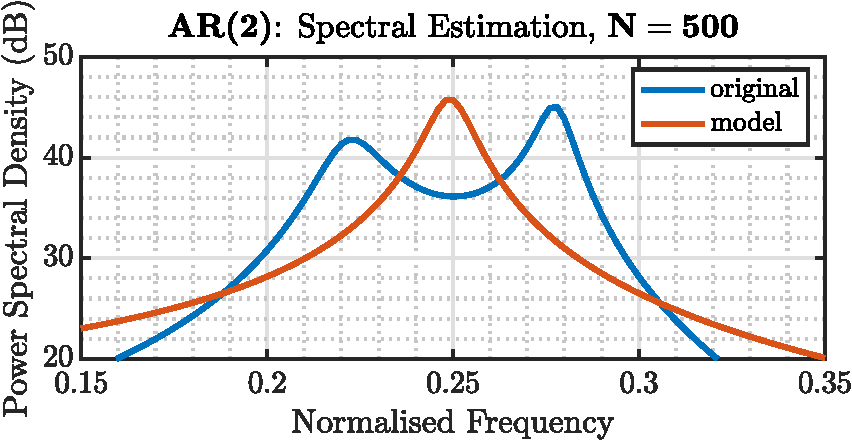
\includegraphics[height=1.5in]{report/parametric-and-line-spectra/spectrum-of-autoregressive-processes/assets/b/ar_2}
    \end{subfigure}
    ~ 
    \begin{subfigure}{0.49\textwidth}
        \centering
        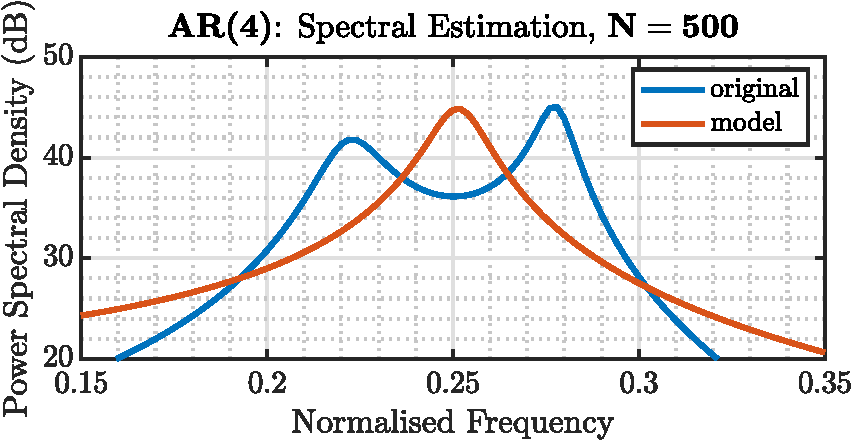
\includegraphics[height=1.5in]{report/parametric-and-line-spectra/spectrum-of-autoregressive-processes/assets/b/ar_4}
    \end{subfigure}
    ~
    ~
    \begin{subfigure}{0.49\textwidth}
        \centering
        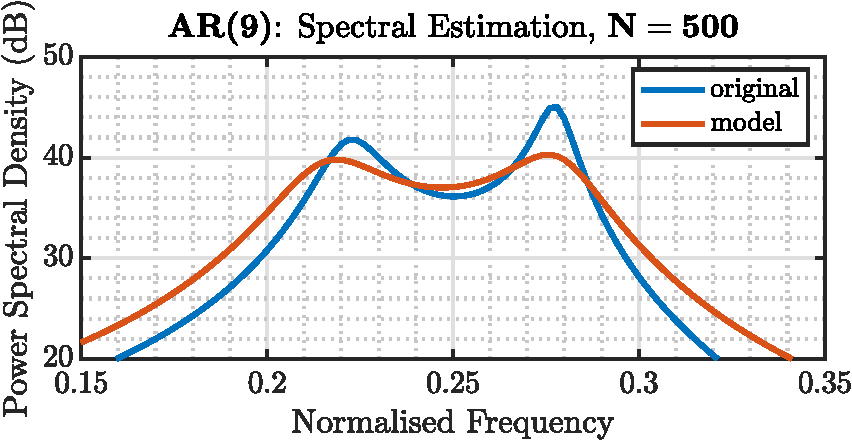
\includegraphics[height=1.5in]{report/parametric-and-line-spectra/spectrum-of-autoregressive-processes/assets/b/ar_9}
    \end{subfigure}
    ~
    \begin{subfigure}{0.49\textwidth}
        \centering
        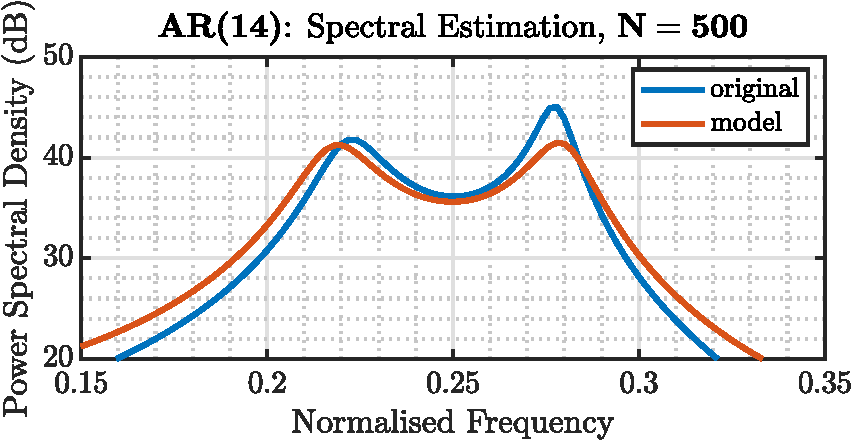
\includegraphics[height=1.5in]{report/parametric-and-line-spectra/spectrum-of-autoregressive-processes/assets/b/ar_14}
    \end{subfigure}
    \caption{AR: spectrum estimates and model order $p$ with $N=500$ samples.}
    \label{fig:2_2_b_1}
\end{figure}

Intuitively, the larger the model order $p$, the more degrees of freedom available to capture the nature of the process.
In figure \ref{fig:2_2_b_2} the noise power (mean squared prediction error) is illustrated as a function of model order $p$.
Unsurprisingly, the error decreases for increasing model order though it plateaus for $p \leq 9$. As a result, to minimize model complexity and avoid fitting error (overfitting)
model order $p = 9$ is selected.

\begin{figure}[h]
    \centering
    \begin{subfigure}{0.49\textwidth}
        \centering
        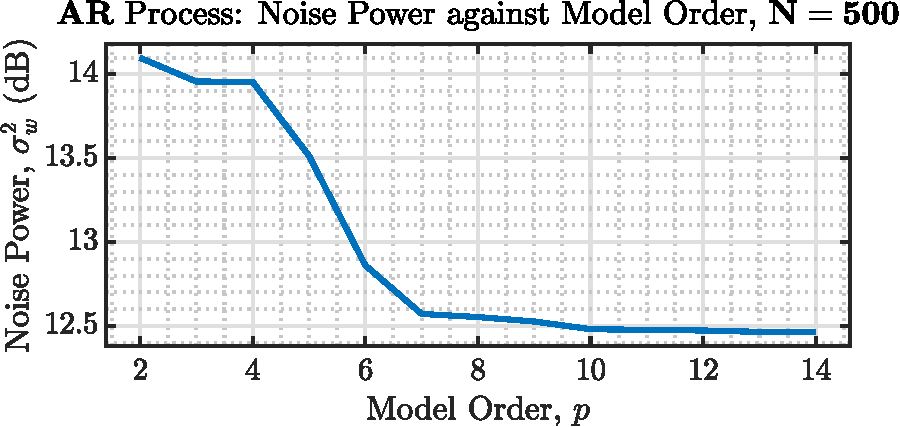
\includegraphics[height=1.5in]{report/parametric-and-line-spectra/spectrum-of-autoregressive-processes/assets/b/error}
    \end{subfigure}
    ~
    \begin{subfigure}{0.49\textwidth}
        \centering
        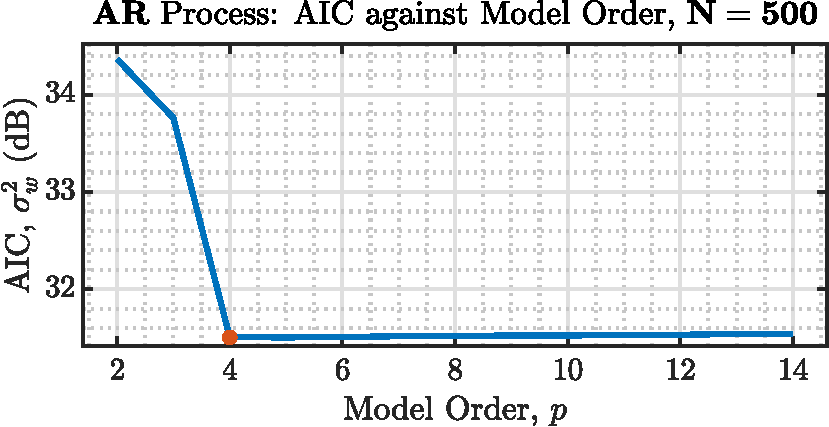
\includegraphics[height=1.5in]{report/parametric-and-line-spectra/spectrum-of-autoregressive-processes/assets/b/aic}
    \end{subfigure}
    \caption{AR: noise power and model order $p$ with $N=500$ samples.}
    \label{fig:2_2_b_2}
\end{figure}

We also highlight that despite the fact that $p_{original} = 4$, due to the small number of available sample ($N = 500$),
when $p = 4$ is selected the fitted model performs very poorly, thus either the number of samples should be increased or a higher order model should be used instead.

%% c)
\item
%

The experiment is repeated for the same AR process, but using $N = 10000$ samples and figures \ref{fig:2_2_c_1} and \ref{fig:2_2_c_2} are obtained.
When $p < p_{original} = 4$, the model still does not have the capacity to model the process (under-modelling) while for $p > p_{original} = 4$ the error plateaus.
Despite the fact that AR(4) model identifies the two peaks, we note that AR(5) and all higher order models track spectrum much better. To avoid overfitting the noise
and preserve generalisation of the model, criteria such as the Akaike Information Criterion (AIC) or the Bayesian Information Criterion can be used to penalise higher order models.
According to the AIC, AR(4) model is selected for this experiment, agreeing with the true model order.

\begin{figure}[h]
    \centering
    \begin{subfigure}{0.49\textwidth}
        \centering
        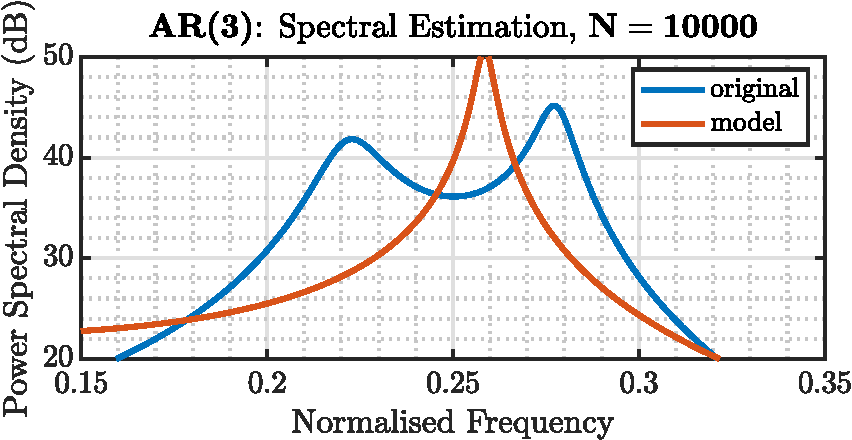
\includegraphics[height=1.5in]{report/parametric-and-line-spectra/spectrum-of-autoregressive-processes/assets/c/ar_3}
    \end{subfigure}
    ~ 
    \begin{subfigure}{0.49\textwidth}
        \centering
        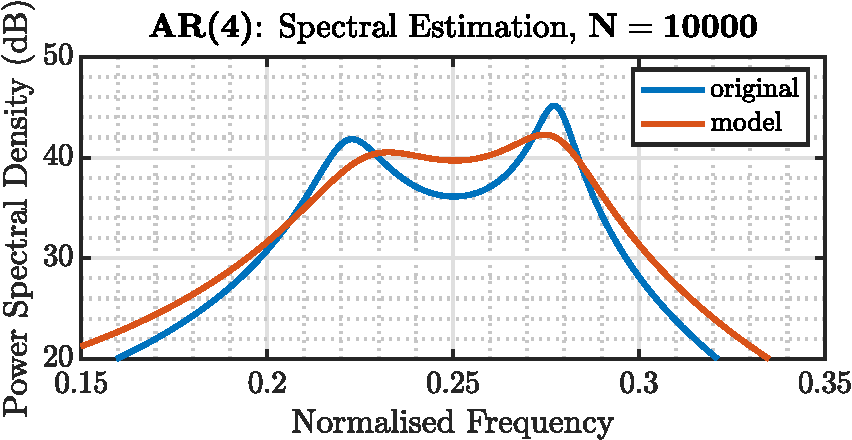
\includegraphics[height=1.5in]{report/parametric-and-line-spectra/spectrum-of-autoregressive-processes/assets/c/ar_4}
    \end{subfigure}
    ~
    ~
    \begin{subfigure}{0.49\textwidth}
        \centering
        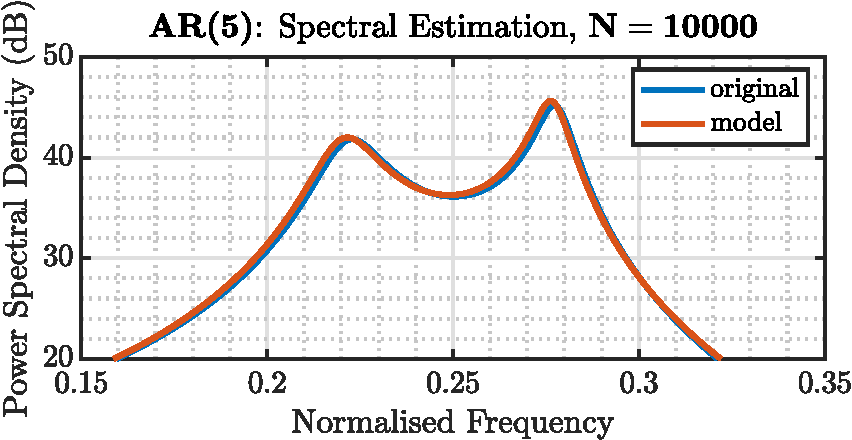
\includegraphics[height=1.5in]{report/parametric-and-line-spectra/spectrum-of-autoregressive-processes/assets/c/ar_5}
    \end{subfigure}
    ~
    \begin{subfigure}{0.49\textwidth}
        \centering
        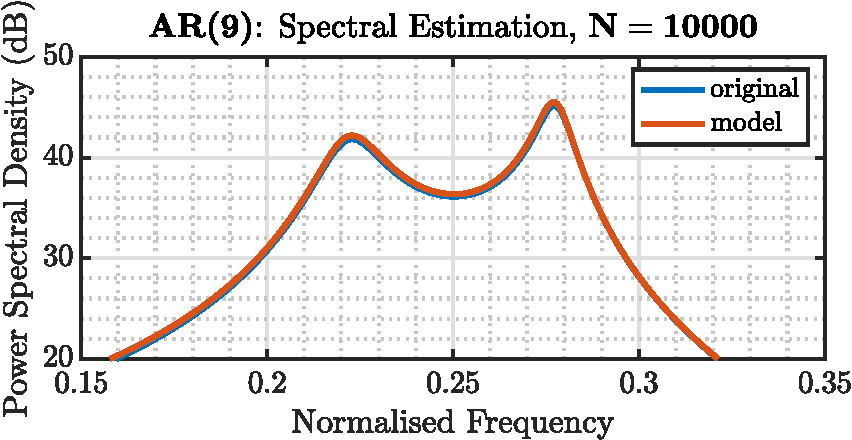
\includegraphics[height=1.5in]{report/parametric-and-line-spectra/spectrum-of-autoregressive-processes/assets/c/ar_9}
    \end{subfigure}
    \caption{AR: spectrum estimates and model order $p$ with $N=10000$ samples.}
    \label{fig:2_2_c_1}
\end{figure}

\begin{figure}[h]
    \centering
    \begin{subfigure}{0.49\textwidth}
        \centering
        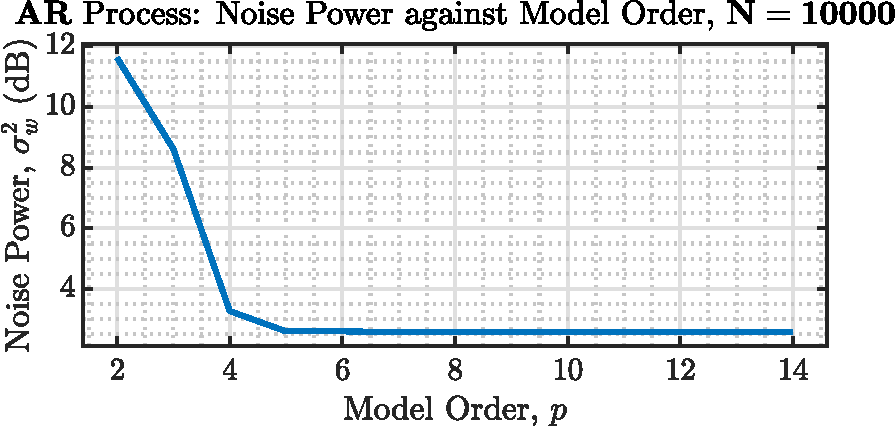
\includegraphics[height=1.5in]{report/parametric-and-line-spectra/spectrum-of-autoregressive-processes/assets/c/error}
    \end{subfigure}
    ~
    \begin{subfigure}{0.49\textwidth}
        \centering
        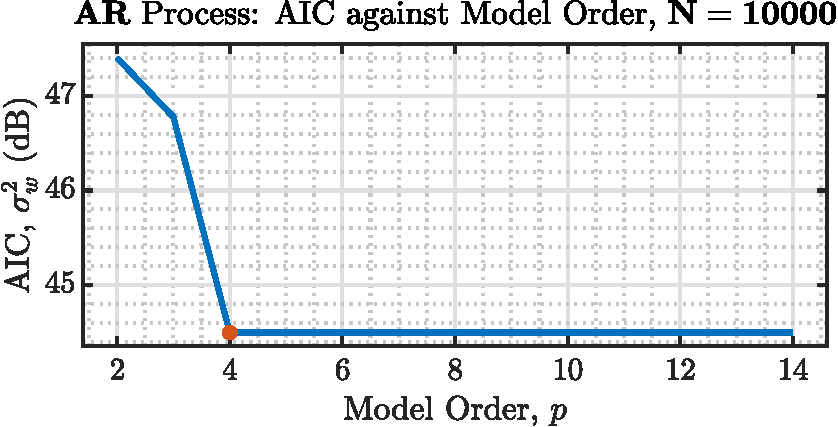
\includegraphics[height=1.5in]{report/parametric-and-line-spectra/spectrum-of-autoregressive-processes/assets/c/aic}
    \end{subfigure}
    \caption{AR: soise power and model order $p$ with $N=10000$ samples.}
    \label{fig:2_2_c_2}
\end{figure}

%
\end{enumerate}
%% Assignment 2
\section{Spectrum of Autoregressive Processes}

\begin{enumerate}[label=\alph*), leftmargin=*]
%% a)
\item
%

A $p$ order Autoregressive process with parameters $\va \in \sR^{p}$ satisfies the Yule-Walker (or normal) equation:

\begin{equation}
    \vr_{xx} = \mathbf{R}_{xx} \va \Rightarrow \va = \mathbf{R}_{xx}^{-1} \vr_{xx}
    \label{eq:yule-walker}
\end{equation}

where $\mathbf{R}_{xx}$ the autocorrelation matrix (ACF) of signal $x(n)$. Equation (\ref{eq:yule-walker}) is meaningful for non-singular and thus invertible $\mathbf{R}_{xx}$.
The biased estimator of ACF guarantees positive semi-definiteness and as a result the $\mathbf{R}_{xx}$ can be inverted, providing solutions for the autoregressive parameters $\va$.
On the other hand, as depicted in figure \ref{fig:2_1_a}, the unbiased ACF estimator leads to indefiniteness and thus $\mathbf{R_{xx}}$ may be singular.

%% b)
\item
%

The power spectral density of an AR process with parameters $\va = [2.76,\ -3.81,\ 2.65,\ -0.92]$ in Guassian white noise ($\sigma^{2} = 1$) is estimated using different AR model order
$p = 2,\ 3,\ \ldots,\ 14$. As illustrated in figure \ref{fig:2_2_b_1}, low order models (i.e $p=2$) fail to capture the behaviour of the process, identifying a single peak in the spectrum,
while two are expected. Higher order models (i.e $p=9$) provide better estimates, able to find the two peaks.

\begin{figure}[h]
    \centering
    \begin{subfigure}{0.49\textwidth}
        \centering
        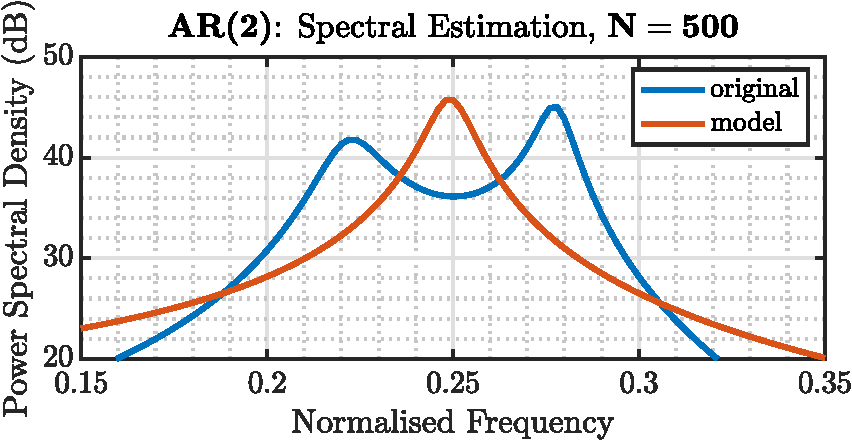
\includegraphics[height=1.5in]{report/parametric-and-line-spectra/spectrum-of-autoregressive-processes/assets/b/ar_2}
    \end{subfigure}
    ~ 
    \begin{subfigure}{0.49\textwidth}
        \centering
        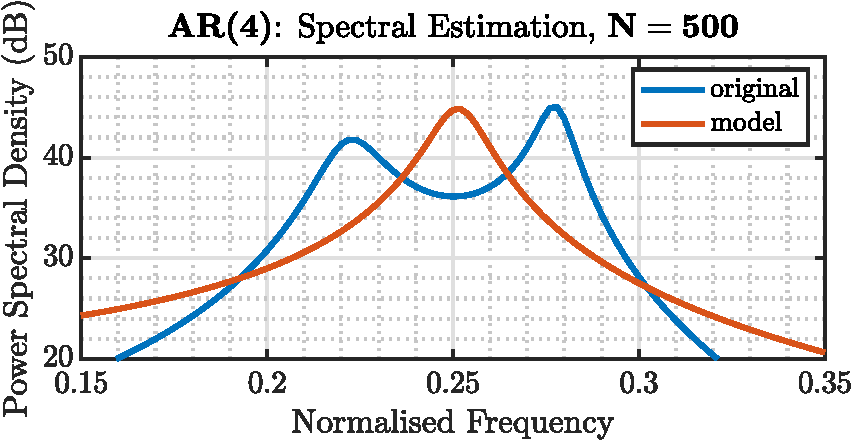
\includegraphics[height=1.5in]{report/parametric-and-line-spectra/spectrum-of-autoregressive-processes/assets/b/ar_4}
    \end{subfigure}
    ~
    ~
    \begin{subfigure}{0.49\textwidth}
        \centering
        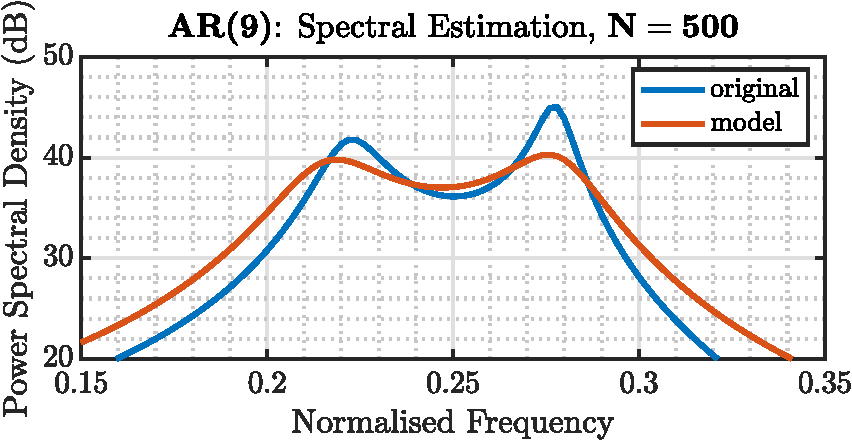
\includegraphics[height=1.5in]{report/parametric-and-line-spectra/spectrum-of-autoregressive-processes/assets/b/ar_9}
    \end{subfigure}
    ~
    \begin{subfigure}{0.49\textwidth}
        \centering
        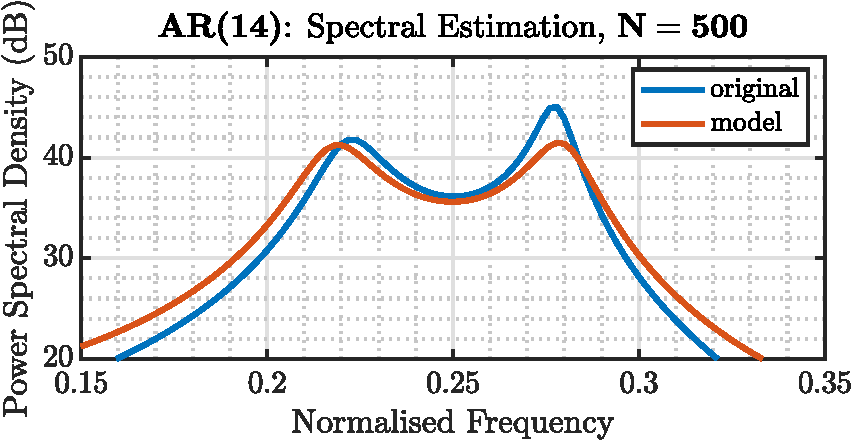
\includegraphics[height=1.5in]{report/parametric-and-line-spectra/spectrum-of-autoregressive-processes/assets/b/ar_14}
    \end{subfigure}
    \caption{AR: spectrum estimates and model order $p$ with $N=500$ samples.}
    \label{fig:2_2_b_1}
\end{figure}

Intuitively, the larger the model order $p$, the more degrees of freedom available to capture the nature of the process.
In figure \ref{fig:2_2_b_2} the noise power (mean squared prediction error) is illustrated as a function of model order $p$.
Unsurprisingly, the error decreases for increasing model order though it plateaus for $p \leq 9$. As a result, to minimize model complexity and avoid fitting error (overfitting)
model order $p = 9$ is selected.

\begin{figure}[h]
    \centering
    \begin{subfigure}{0.49\textwidth}
        \centering
        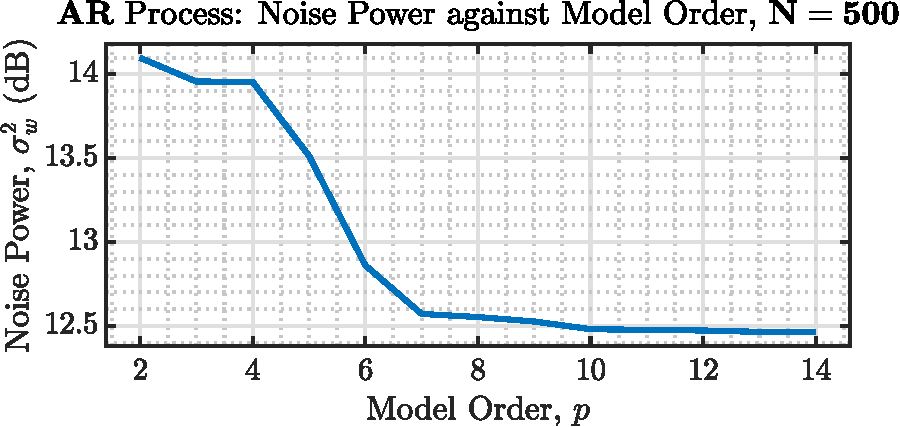
\includegraphics[height=1.5in]{report/parametric-and-line-spectra/spectrum-of-autoregressive-processes/assets/b/error}
    \end{subfigure}
    ~
    \begin{subfigure}{0.49\textwidth}
        \centering
        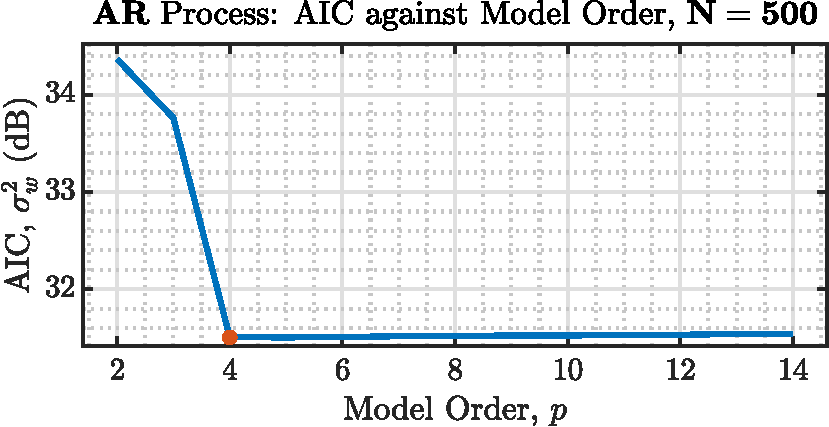
\includegraphics[height=1.5in]{report/parametric-and-line-spectra/spectrum-of-autoregressive-processes/assets/b/aic}
    \end{subfigure}
    \caption{AR: noise power and model order $p$ with $N=500$ samples.}
    \label{fig:2_2_b_2}
\end{figure}

We also highlight that despite the fact that $p_{original} = 4$, due to the small number of available sample ($N = 500$),
when $p = 4$ is selected the fitted model performs very poorly, thus either the number of samples should be increased or a higher order model should be used instead.

%% c)
\item
%

The experiment is repeated for the same AR process, but using $N = 10000$ samples and figures \ref{fig:2_2_c_1} and \ref{fig:2_2_c_2} are obtained.
When $p < p_{original} = 4$, the model still does not have the capacity to model the process (under-modelling) while for $p > p_{original} = 4$ the error plateaus.
Despite the fact that AR(4) model identifies the two peaks, we note that AR(5) and all higher order models track spectrum much better. To avoid overfitting the noise
and preserve generalisation of the model, criteria such as the Akaike Information Criterion (AIC) or the Bayesian Information Criterion can be used to penalise higher order models.
According to the AIC, AR(4) model is selected for this experiment, agreeing with the true model order.

\begin{figure}[h]
    \centering
    \begin{subfigure}{0.49\textwidth}
        \centering
        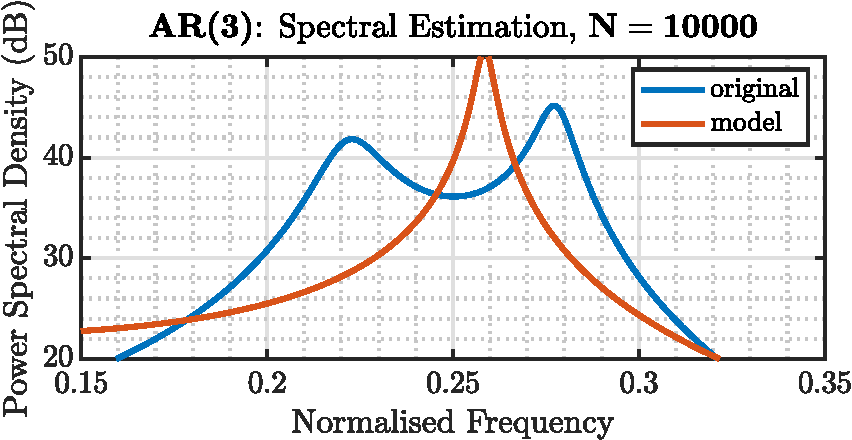
\includegraphics[height=1.5in]{report/parametric-and-line-spectra/spectrum-of-autoregressive-processes/assets/c/ar_3}
    \end{subfigure}
    ~ 
    \begin{subfigure}{0.49\textwidth}
        \centering
        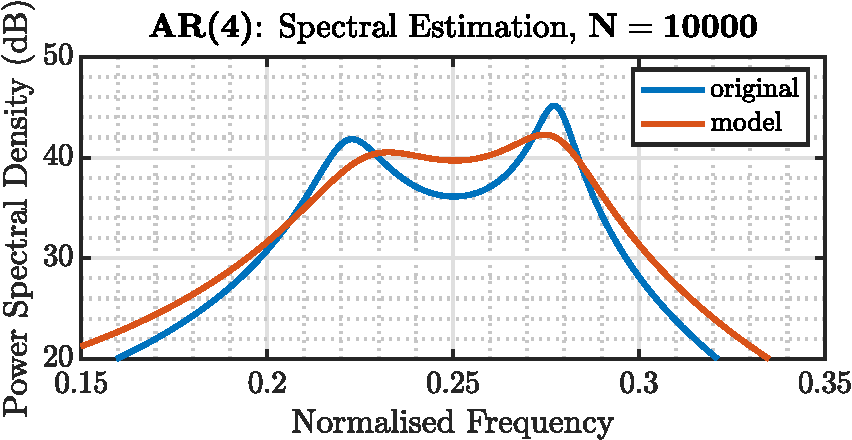
\includegraphics[height=1.5in]{report/parametric-and-line-spectra/spectrum-of-autoregressive-processes/assets/c/ar_4}
    \end{subfigure}
    ~
    ~
    \begin{subfigure}{0.49\textwidth}
        \centering
        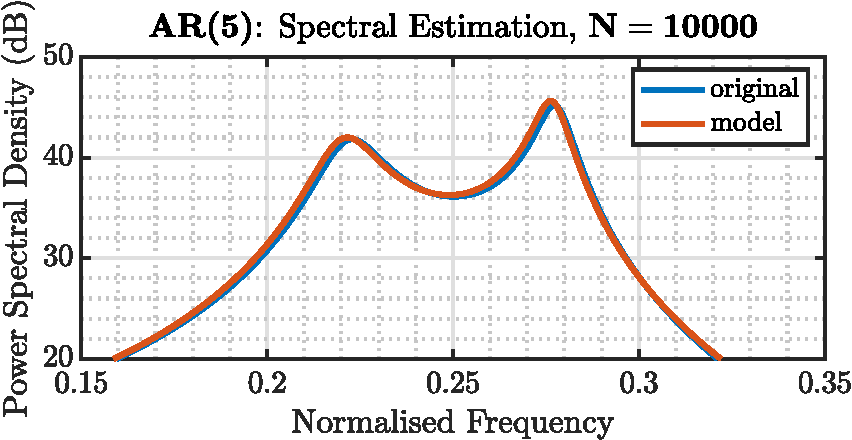
\includegraphics[height=1.5in]{report/parametric-and-line-spectra/spectrum-of-autoregressive-processes/assets/c/ar_5}
    \end{subfigure}
    ~
    \begin{subfigure}{0.49\textwidth}
        \centering
        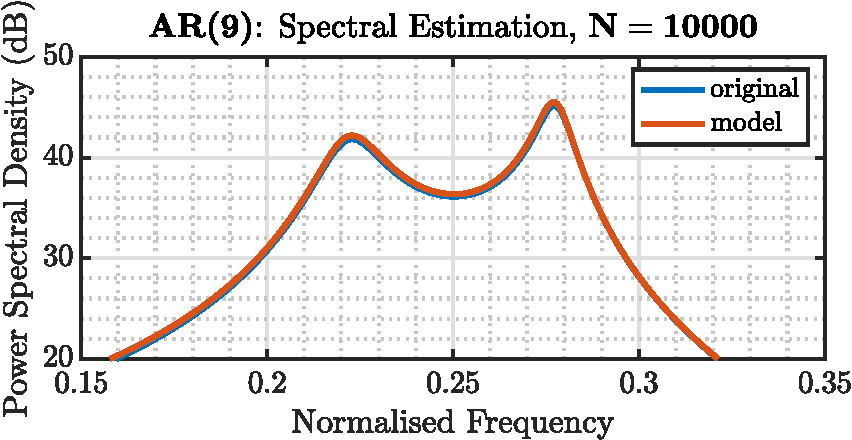
\includegraphics[height=1.5in]{report/parametric-and-line-spectra/spectrum-of-autoregressive-processes/assets/c/ar_9}
    \end{subfigure}
    \caption{AR: spectrum estimates and model order $p$ with $N=10000$ samples.}
    \label{fig:2_2_c_1}
\end{figure}

\begin{figure}[h]
    \centering
    \begin{subfigure}{0.49\textwidth}
        \centering
        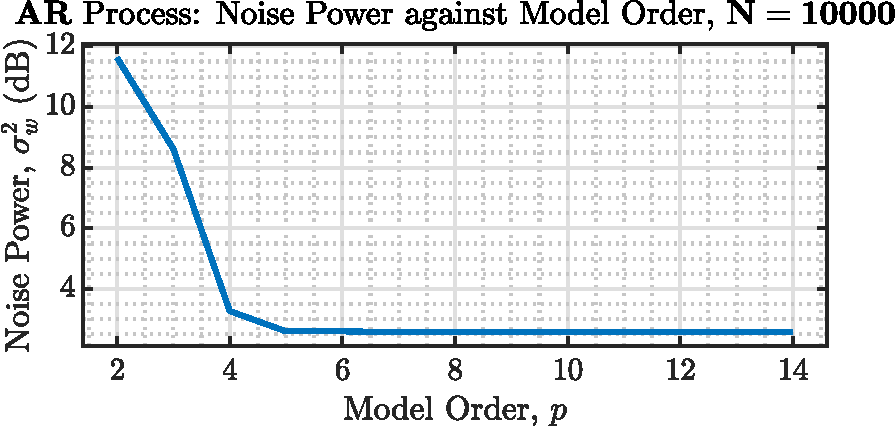
\includegraphics[height=1.5in]{report/parametric-and-line-spectra/spectrum-of-autoregressive-processes/assets/c/error}
    \end{subfigure}
    ~
    \begin{subfigure}{0.49\textwidth}
        \centering
        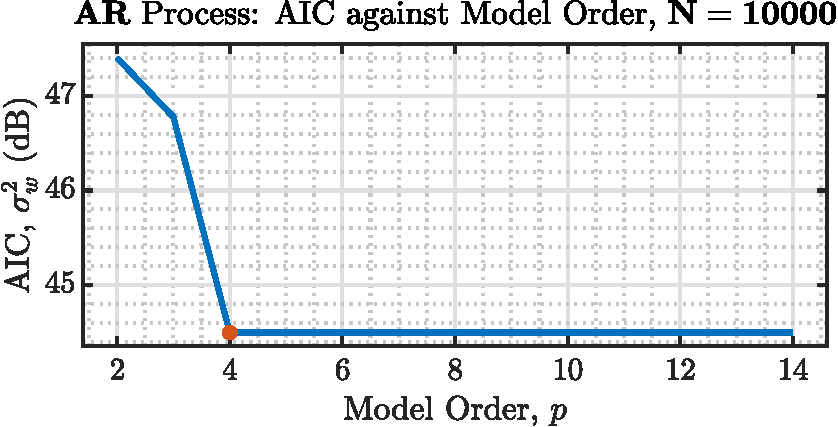
\includegraphics[height=1.5in]{report/parametric-and-line-spectra/spectrum-of-autoregressive-processes/assets/c/aic}
    \end{subfigure}
    \caption{AR: soise power and model order $p$ with $N=10000$ samples.}
    \label{fig:2_2_c_2}
\end{figure}

%
\end{enumerate}
%% Assignment 3
\section{Spectrum of Autoregressive Processes}

\begin{enumerate}[label=\alph*), leftmargin=*]
%% a)
\item
%

A $p$ order Autoregressive process with parameters $\va \in \sR^{p}$ satisfies the Yule-Walker (or normal) equation:

\begin{equation}
    \vr_{xx} = \mathbf{R}_{xx} \va \Rightarrow \va = \mathbf{R}_{xx}^{-1} \vr_{xx}
    \label{eq:yule-walker}
\end{equation}

where $\mathbf{R}_{xx}$ the autocorrelation matrix (ACF) of signal $x(n)$. Equation (\ref{eq:yule-walker}) is meaningful for non-singular and thus invertible $\mathbf{R}_{xx}$.
The biased estimator of ACF guarantees positive semi-definiteness and as a result the $\mathbf{R}_{xx}$ can be inverted, providing solutions for the autoregressive parameters $\va$.
On the other hand, as depicted in figure \ref{fig:2_1_a}, the unbiased ACF estimator leads to indefiniteness and thus $\mathbf{R_{xx}}$ may be singular.

%% b)
\item
%

The power spectral density of an AR process with parameters $\va = [2.76,\ -3.81,\ 2.65,\ -0.92]$ in Guassian white noise ($\sigma^{2} = 1$) is estimated using different AR model order
$p = 2,\ 3,\ \ldots,\ 14$. As illustrated in figure \ref{fig:2_2_b_1}, low order models (i.e $p=2$) fail to capture the behaviour of the process, identifying a single peak in the spectrum,
while two are expected. Higher order models (i.e $p=9$) provide better estimates, able to find the two peaks.

\begin{figure}[h]
    \centering
    \begin{subfigure}{0.49\textwidth}
        \centering
        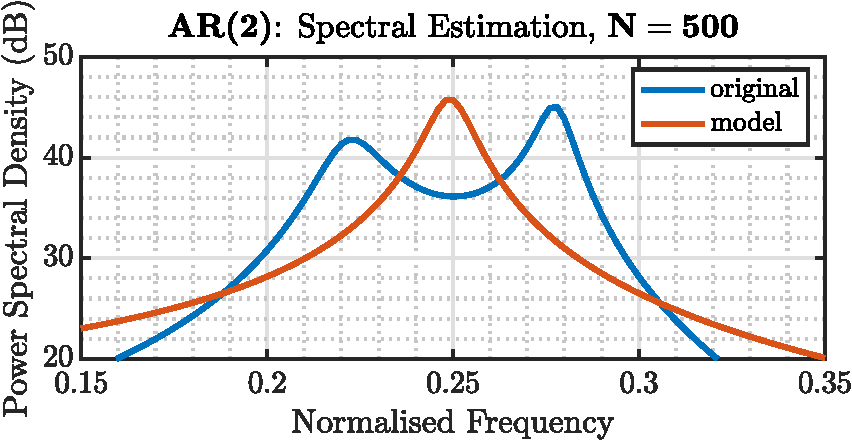
\includegraphics[height=1.5in]{report/parametric-and-line-spectra/spectrum-of-autoregressive-processes/assets/b/ar_2}
    \end{subfigure}
    ~ 
    \begin{subfigure}{0.49\textwidth}
        \centering
        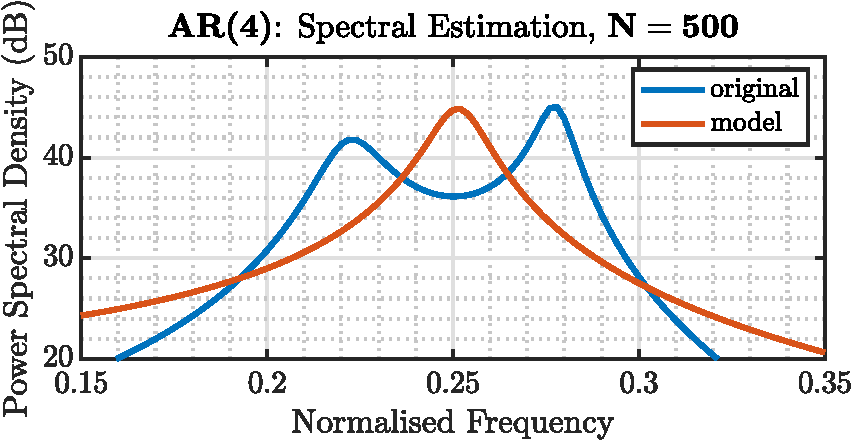
\includegraphics[height=1.5in]{report/parametric-and-line-spectra/spectrum-of-autoregressive-processes/assets/b/ar_4}
    \end{subfigure}
    ~
    ~
    \begin{subfigure}{0.49\textwidth}
        \centering
        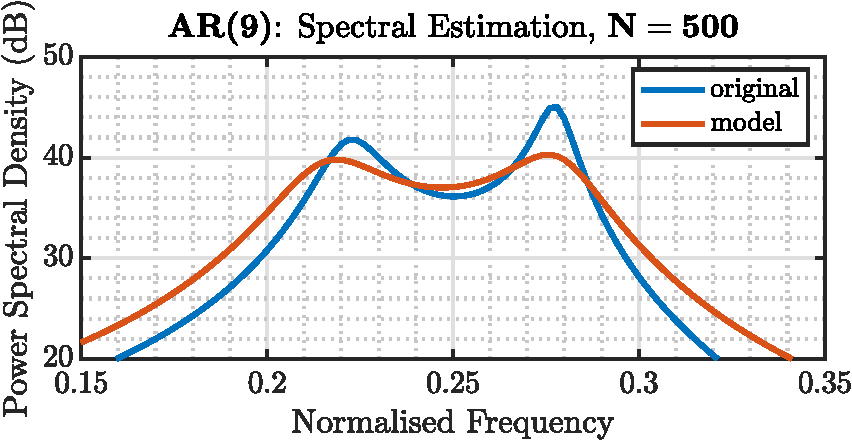
\includegraphics[height=1.5in]{report/parametric-and-line-spectra/spectrum-of-autoregressive-processes/assets/b/ar_9}
    \end{subfigure}
    ~
    \begin{subfigure}{0.49\textwidth}
        \centering
        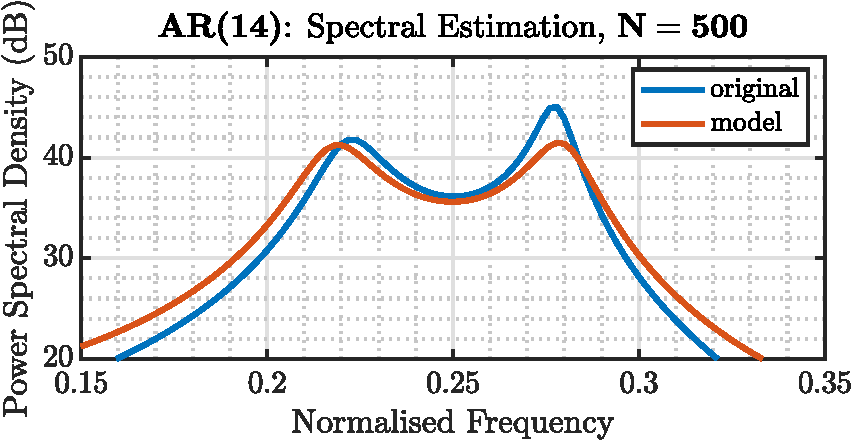
\includegraphics[height=1.5in]{report/parametric-and-line-spectra/spectrum-of-autoregressive-processes/assets/b/ar_14}
    \end{subfigure}
    \caption{AR: spectrum estimates and model order $p$ with $N=500$ samples.}
    \label{fig:2_2_b_1}
\end{figure}

Intuitively, the larger the model order $p$, the more degrees of freedom available to capture the nature of the process.
In figure \ref{fig:2_2_b_2} the noise power (mean squared prediction error) is illustrated as a function of model order $p$.
Unsurprisingly, the error decreases for increasing model order though it plateaus for $p \leq 9$. As a result, to minimize model complexity and avoid fitting error (overfitting)
model order $p = 9$ is selected.

\begin{figure}[h]
    \centering
    \begin{subfigure}{0.49\textwidth}
        \centering
        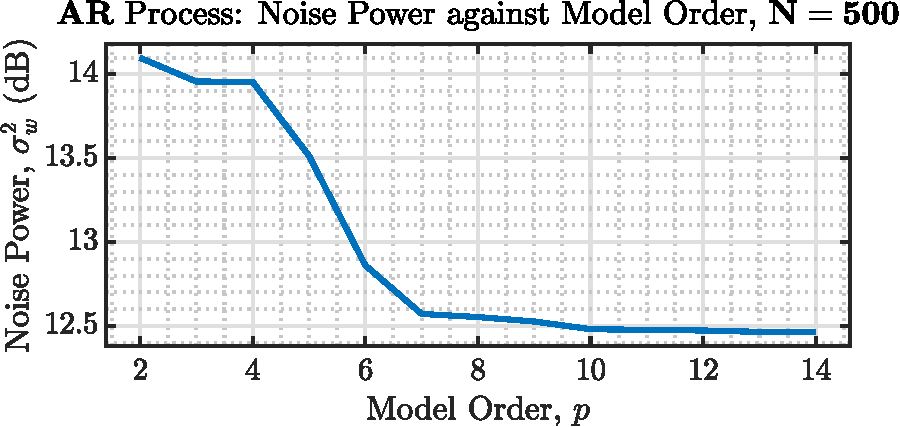
\includegraphics[height=1.5in]{report/parametric-and-line-spectra/spectrum-of-autoregressive-processes/assets/b/error}
    \end{subfigure}
    ~
    \begin{subfigure}{0.49\textwidth}
        \centering
        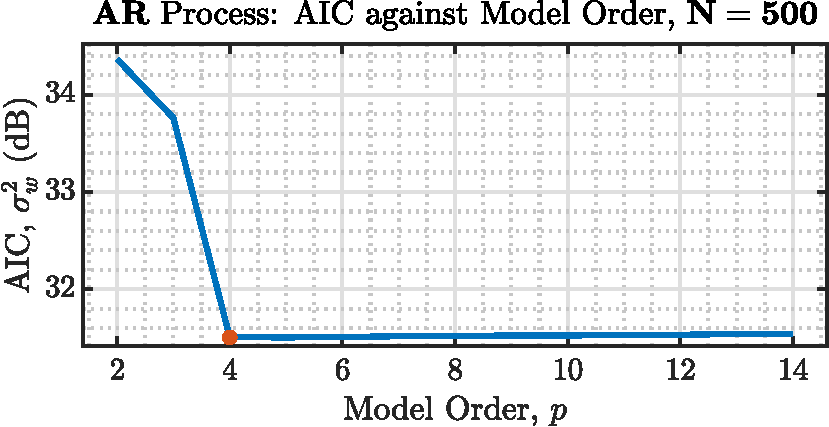
\includegraphics[height=1.5in]{report/parametric-and-line-spectra/spectrum-of-autoregressive-processes/assets/b/aic}
    \end{subfigure}
    \caption{AR: noise power and model order $p$ with $N=500$ samples.}
    \label{fig:2_2_b_2}
\end{figure}

We also highlight that despite the fact that $p_{original} = 4$, due to the small number of available sample ($N = 500$),
when $p = 4$ is selected the fitted model performs very poorly, thus either the number of samples should be increased or a higher order model should be used instead.

%% c)
\item
%

The experiment is repeated for the same AR process, but using $N = 10000$ samples and figures \ref{fig:2_2_c_1} and \ref{fig:2_2_c_2} are obtained.
When $p < p_{original} = 4$, the model still does not have the capacity to model the process (under-modelling) while for $p > p_{original} = 4$ the error plateaus.
Despite the fact that AR(4) model identifies the two peaks, we note that AR(5) and all higher order models track spectrum much better. To avoid overfitting the noise
and preserve generalisation of the model, criteria such as the Akaike Information Criterion (AIC) or the Bayesian Information Criterion can be used to penalise higher order models.
According to the AIC, AR(4) model is selected for this experiment, agreeing with the true model order.

\begin{figure}[h]
    \centering
    \begin{subfigure}{0.49\textwidth}
        \centering
        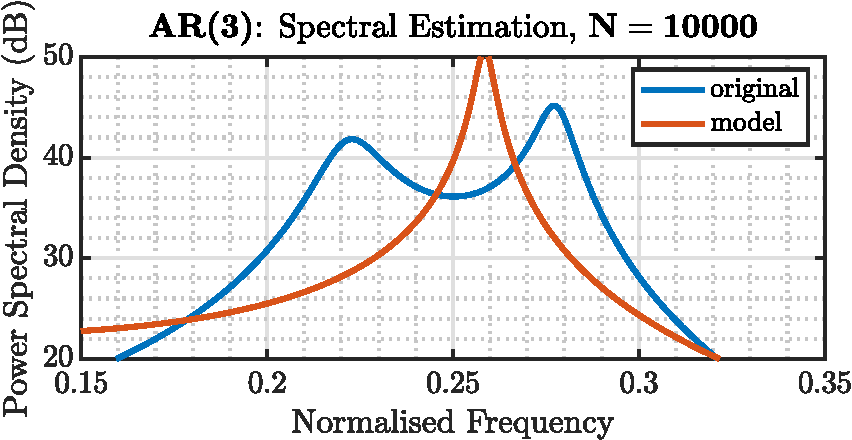
\includegraphics[height=1.5in]{report/parametric-and-line-spectra/spectrum-of-autoregressive-processes/assets/c/ar_3}
    \end{subfigure}
    ~ 
    \begin{subfigure}{0.49\textwidth}
        \centering
        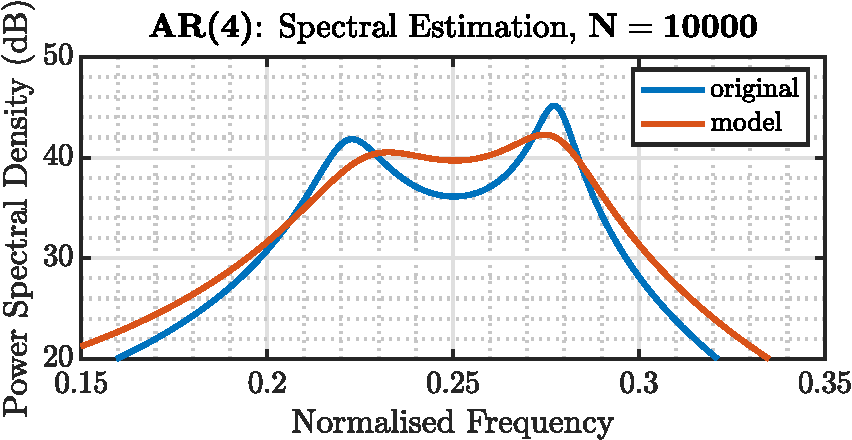
\includegraphics[height=1.5in]{report/parametric-and-line-spectra/spectrum-of-autoregressive-processes/assets/c/ar_4}
    \end{subfigure}
    ~
    ~
    \begin{subfigure}{0.49\textwidth}
        \centering
        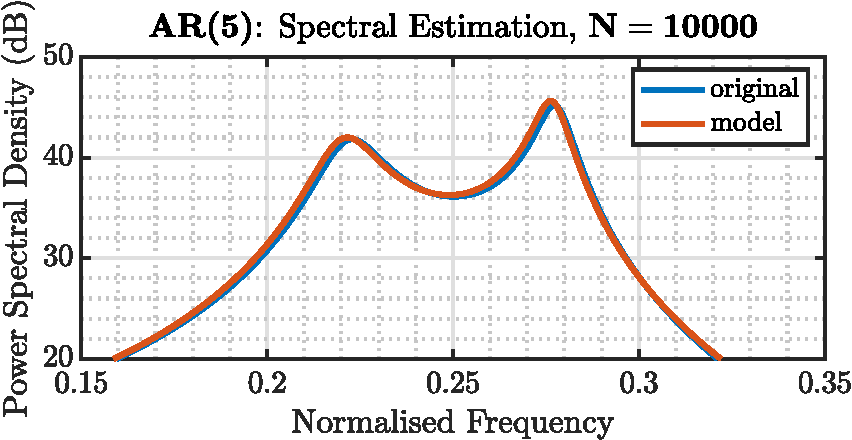
\includegraphics[height=1.5in]{report/parametric-and-line-spectra/spectrum-of-autoregressive-processes/assets/c/ar_5}
    \end{subfigure}
    ~
    \begin{subfigure}{0.49\textwidth}
        \centering
        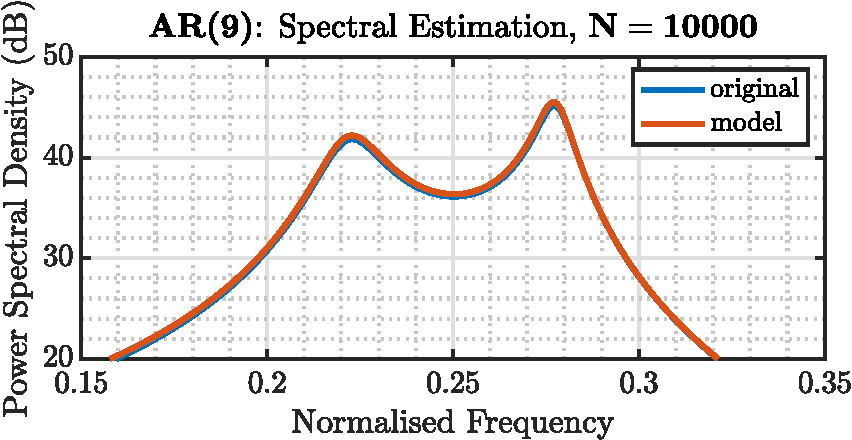
\includegraphics[height=1.5in]{report/parametric-and-line-spectra/spectrum-of-autoregressive-processes/assets/c/ar_9}
    \end{subfigure}
    \caption{AR: spectrum estimates and model order $p$ with $N=10000$ samples.}
    \label{fig:2_2_c_1}
\end{figure}

\begin{figure}[h]
    \centering
    \begin{subfigure}{0.49\textwidth}
        \centering
        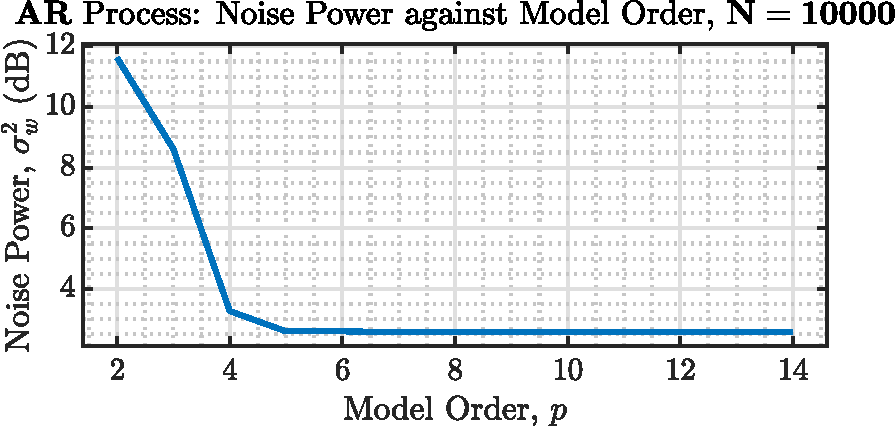
\includegraphics[height=1.5in]{report/parametric-and-line-spectra/spectrum-of-autoregressive-processes/assets/c/error}
    \end{subfigure}
    ~
    \begin{subfigure}{0.49\textwidth}
        \centering
        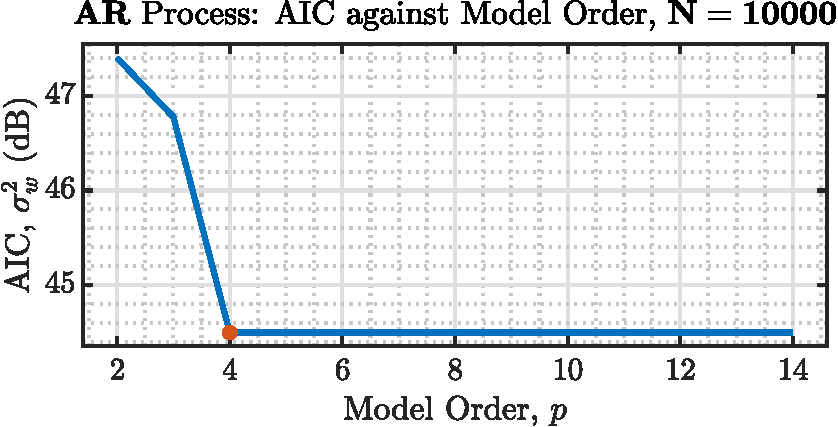
\includegraphics[height=1.5in]{report/parametric-and-line-spectra/spectrum-of-autoregressive-processes/assets/c/aic}
    \end{subfigure}
    \caption{AR: soise power and model order $p$ with $N=10000$ samples.}
    \label{fig:2_2_c_2}
\end{figure}

%
\end{enumerate}
%% Assignment 4
\section{Spectrum of Autoregressive Processes}

\begin{enumerate}[label=\alph*), leftmargin=*]
%% a)
\item
%

A $p$ order Autoregressive process with parameters $\va \in \sR^{p}$ satisfies the Yule-Walker (or normal) equation:

\begin{equation}
    \vr_{xx} = \mathbf{R}_{xx} \va \Rightarrow \va = \mathbf{R}_{xx}^{-1} \vr_{xx}
    \label{eq:yule-walker}
\end{equation}

where $\mathbf{R}_{xx}$ the autocorrelation matrix (ACF) of signal $x(n)$. Equation (\ref{eq:yule-walker}) is meaningful for non-singular and thus invertible $\mathbf{R}_{xx}$.
The biased estimator of ACF guarantees positive semi-definiteness and as a result the $\mathbf{R}_{xx}$ can be inverted, providing solutions for the autoregressive parameters $\va$.
On the other hand, as depicted in figure \ref{fig:2_1_a}, the unbiased ACF estimator leads to indefiniteness and thus $\mathbf{R_{xx}}$ may be singular.

%% b)
\item
%

The power spectral density of an AR process with parameters $\va = [2.76,\ -3.81,\ 2.65,\ -0.92]$ in Guassian white noise ($\sigma^{2} = 1$) is estimated using different AR model order
$p = 2,\ 3,\ \ldots,\ 14$. As illustrated in figure \ref{fig:2_2_b_1}, low order models (i.e $p=2$) fail to capture the behaviour of the process, identifying a single peak in the spectrum,
while two are expected. Higher order models (i.e $p=9$) provide better estimates, able to find the two peaks.

\begin{figure}[h]
    \centering
    \begin{subfigure}{0.49\textwidth}
        \centering
        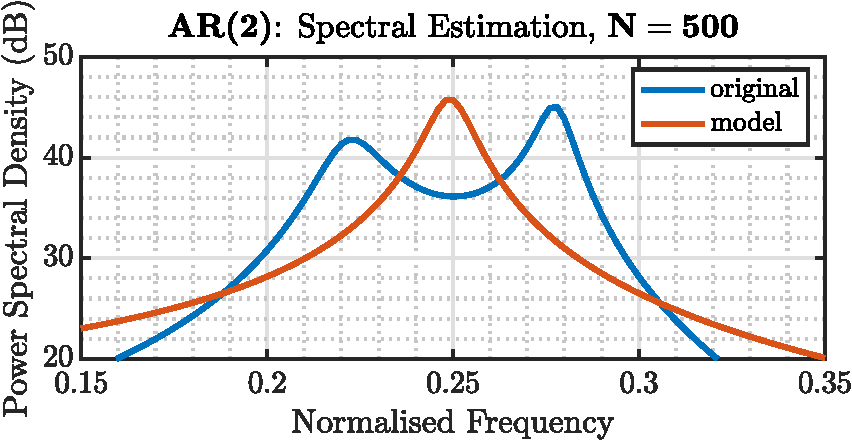
\includegraphics[height=1.5in]{report/parametric-and-line-spectra/spectrum-of-autoregressive-processes/assets/b/ar_2}
    \end{subfigure}
    ~ 
    \begin{subfigure}{0.49\textwidth}
        \centering
        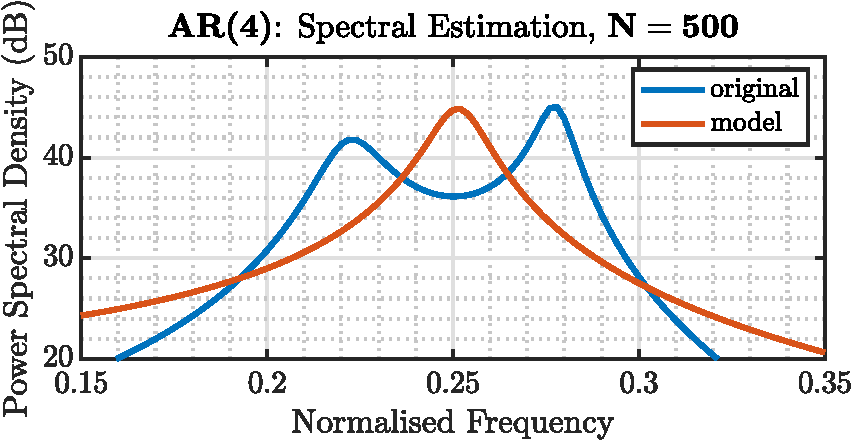
\includegraphics[height=1.5in]{report/parametric-and-line-spectra/spectrum-of-autoregressive-processes/assets/b/ar_4}
    \end{subfigure}
    ~
    ~
    \begin{subfigure}{0.49\textwidth}
        \centering
        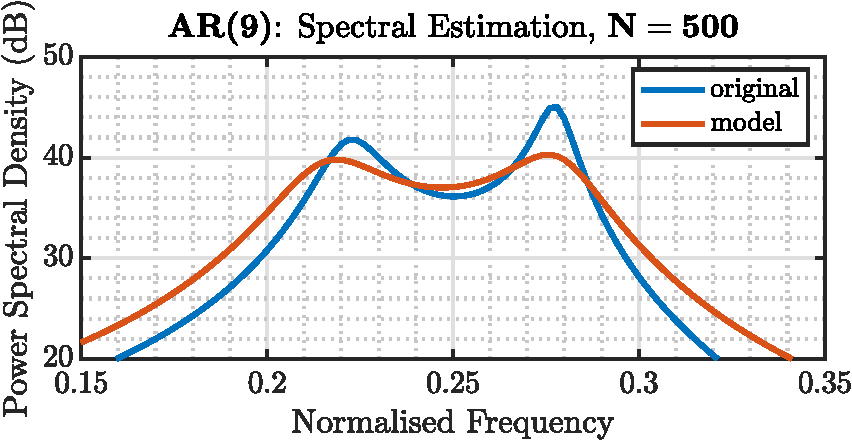
\includegraphics[height=1.5in]{report/parametric-and-line-spectra/spectrum-of-autoregressive-processes/assets/b/ar_9}
    \end{subfigure}
    ~
    \begin{subfigure}{0.49\textwidth}
        \centering
        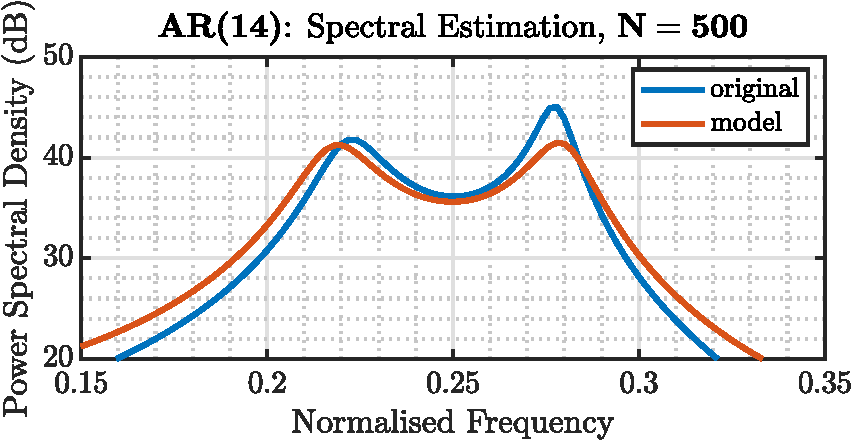
\includegraphics[height=1.5in]{report/parametric-and-line-spectra/spectrum-of-autoregressive-processes/assets/b/ar_14}
    \end{subfigure}
    \caption{AR: spectrum estimates and model order $p$ with $N=500$ samples.}
    \label{fig:2_2_b_1}
\end{figure}

Intuitively, the larger the model order $p$, the more degrees of freedom available to capture the nature of the process.
In figure \ref{fig:2_2_b_2} the noise power (mean squared prediction error) is illustrated as a function of model order $p$.
Unsurprisingly, the error decreases for increasing model order though it plateaus for $p \leq 9$. As a result, to minimize model complexity and avoid fitting error (overfitting)
model order $p = 9$ is selected.

\begin{figure}[h]
    \centering
    \begin{subfigure}{0.49\textwidth}
        \centering
        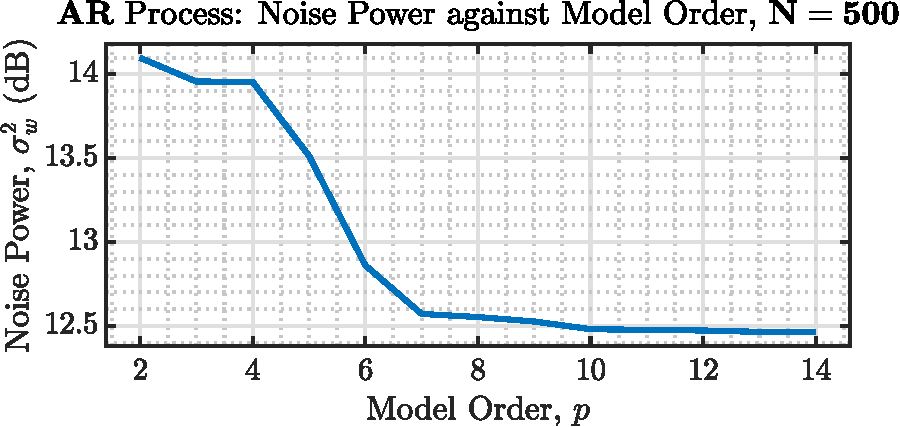
\includegraphics[height=1.5in]{report/parametric-and-line-spectra/spectrum-of-autoregressive-processes/assets/b/error}
    \end{subfigure}
    ~
    \begin{subfigure}{0.49\textwidth}
        \centering
        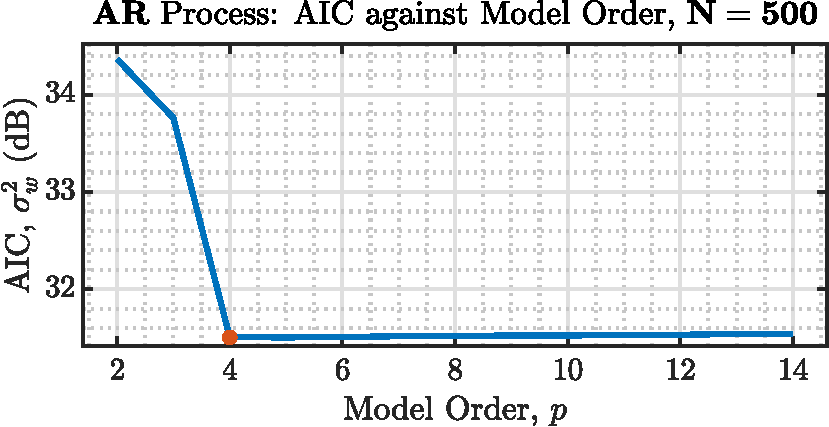
\includegraphics[height=1.5in]{report/parametric-and-line-spectra/spectrum-of-autoregressive-processes/assets/b/aic}
    \end{subfigure}
    \caption{AR: noise power and model order $p$ with $N=500$ samples.}
    \label{fig:2_2_b_2}
\end{figure}

We also highlight that despite the fact that $p_{original} = 4$, due to the small number of available sample ($N = 500$),
when $p = 4$ is selected the fitted model performs very poorly, thus either the number of samples should be increased or a higher order model should be used instead.

%% c)
\item
%

The experiment is repeated for the same AR process, but using $N = 10000$ samples and figures \ref{fig:2_2_c_1} and \ref{fig:2_2_c_2} are obtained.
When $p < p_{original} = 4$, the model still does not have the capacity to model the process (under-modelling) while for $p > p_{original} = 4$ the error plateaus.
Despite the fact that AR(4) model identifies the two peaks, we note that AR(5) and all higher order models track spectrum much better. To avoid overfitting the noise
and preserve generalisation of the model, criteria such as the Akaike Information Criterion (AIC) or the Bayesian Information Criterion can be used to penalise higher order models.
According to the AIC, AR(4) model is selected for this experiment, agreeing with the true model order.

\begin{figure}[h]
    \centering
    \begin{subfigure}{0.49\textwidth}
        \centering
        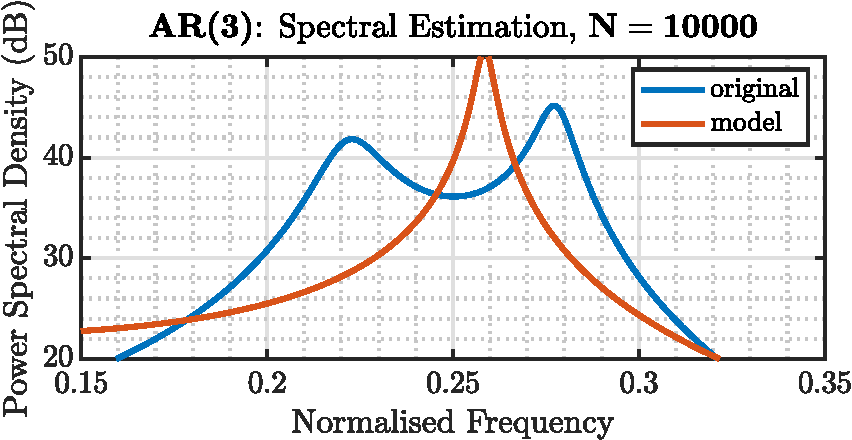
\includegraphics[height=1.5in]{report/parametric-and-line-spectra/spectrum-of-autoregressive-processes/assets/c/ar_3}
    \end{subfigure}
    ~ 
    \begin{subfigure}{0.49\textwidth}
        \centering
        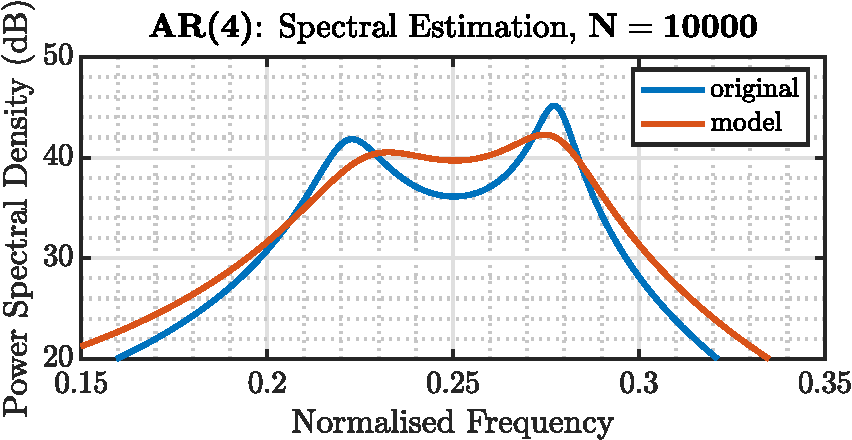
\includegraphics[height=1.5in]{report/parametric-and-line-spectra/spectrum-of-autoregressive-processes/assets/c/ar_4}
    \end{subfigure}
    ~
    ~
    \begin{subfigure}{0.49\textwidth}
        \centering
        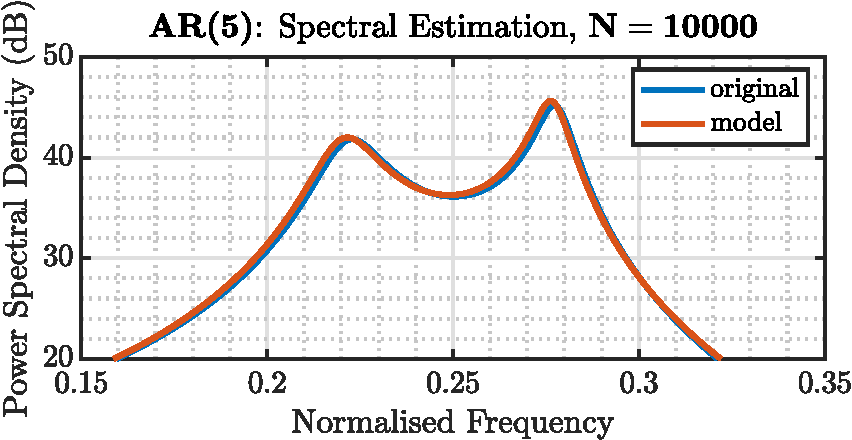
\includegraphics[height=1.5in]{report/parametric-and-line-spectra/spectrum-of-autoregressive-processes/assets/c/ar_5}
    \end{subfigure}
    ~
    \begin{subfigure}{0.49\textwidth}
        \centering
        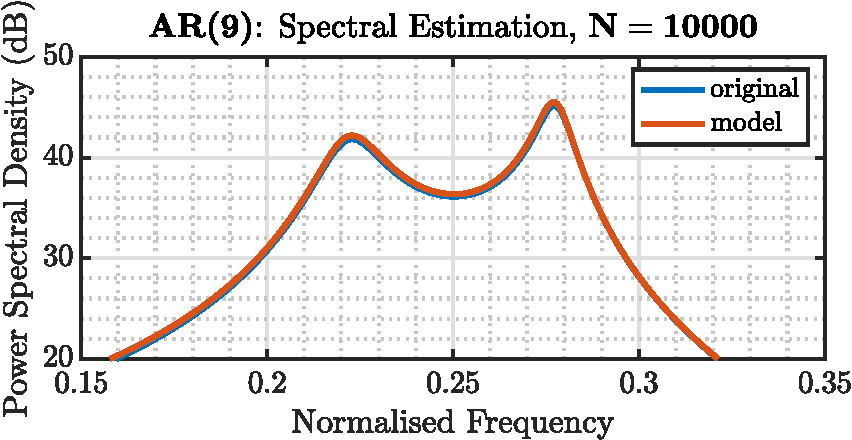
\includegraphics[height=1.5in]{report/parametric-and-line-spectra/spectrum-of-autoregressive-processes/assets/c/ar_9}
    \end{subfigure}
    \caption{AR: spectrum estimates and model order $p$ with $N=10000$ samples.}
    \label{fig:2_2_c_1}
\end{figure}

\begin{figure}[h]
    \centering
    \begin{subfigure}{0.49\textwidth}
        \centering
        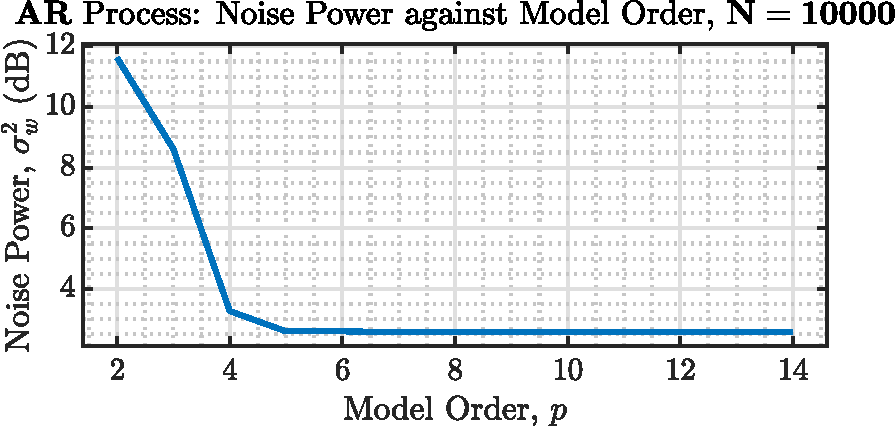
\includegraphics[height=1.5in]{report/parametric-and-line-spectra/spectrum-of-autoregressive-processes/assets/c/error}
    \end{subfigure}
    ~
    \begin{subfigure}{0.49\textwidth}
        \centering
        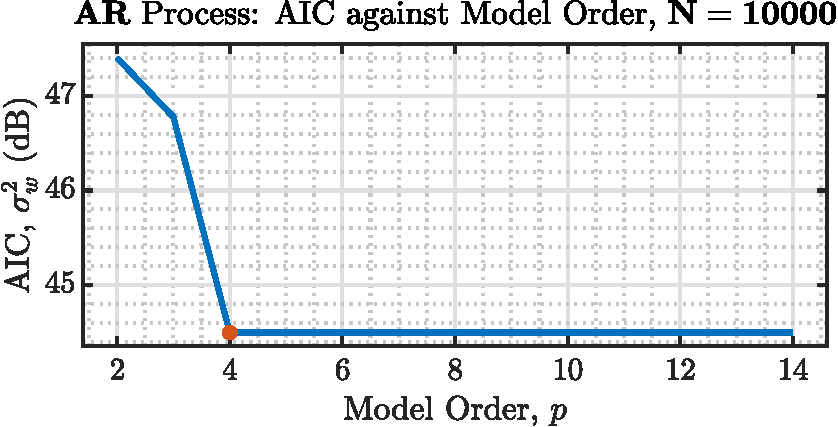
\includegraphics[height=1.5in]{report/parametric-and-line-spectra/spectrum-of-autoregressive-processes/assets/c/aic}
    \end{subfigure}
    \caption{AR: soise power and model order $p$ with $N=10000$ samples.}
    \label{fig:2_2_c_2}
\end{figure}

%
\end{enumerate}


\backmatter

\printbibliography

\end{document}
